\pdfbookmark{Общая характеристика работы}{characteristic}             % Закладка pdf
\section*{Общая характеристика работы}

\newcommand{\actuality}{\pdfbookmark[1]{Актуальность}{actuality}\underline{\textbf{\actualityTXT}}}
\newcommand{\progress}{\pdfbookmark[1]{Разработанность темы}{progress}\underline{\textbf{\progressTXT}}}
\newcommand{\aim}{\pdfbookmark[1]{Цели}{aim}\underline{{\textbf\aimTXT}}}
\newcommand{\tasks}{\pdfbookmark[1]{Задачи}{tasks}\underline{\textbf{\tasksTXT}}}
\newcommand{\aimtasks}{\pdfbookmark[1]{Цели и задачи}{aimtasks}\aimtasksTXT}
\newcommand{\novelty}{\pdfbookmark[1]{Научная новизна}{novelty}\underline{\textbf{\noveltyTXT}}}
\newcommand{\influence}{\pdfbookmark[1]{Практическая значимость}{influence}\underline{\textbf{\influenceTXT}}}
\newcommand{\methods}{\pdfbookmark[1]{Методология и методы исследования}{methods}\underline{\textbf{\methodsTXT}}}
\newcommand{\defpositions}{\pdfbookmark[1]{Положения, выносимые на защиту}{defpositions}\underline{\textbf{\defpositionsTXT}}}
\newcommand{\reliability}{\pdfbookmark[1]{Достоверность}{reliability}\underline{\textbf{\reliabilityTXT}}}
\newcommand{\probation}{\pdfbookmark[1]{Апробация}{probation}\underline{\textbf{\probationTXT}}}
\newcommand{\contribution}{\pdfbookmark[1]{Личный вклад}{contribution}\underline{\textbf{\contributionTXT}}}
\newcommand{\publications}{\pdfbookmark[1]{Публикации}{publications}\underline{\textbf{\publicationsTXT}}}

\newcommand{\realisation}{\underline{\textbf{\realisationTXT}}}


{\actuality} На борту космических аппаратов различного назначения устанавливаются приборы и устройства, содержащие вращающиеся элементы с электроприводом. К таким устройствам относятся поворотные панели солнечных батарей, сканирующие зеркала и оптико-электронные системы дистанционного зондирования Земли, обеспечивающие наведение оптической оси в заданное направление и непрерывное сканирование исследуемого пространства во время движения аппарата по орбите.

В соответствии с третьим законом Ньютона момент, развиваемый электродвигателем, прикладывается не только к ротору, но и к статору (реактивный момент), который через систему крепления передаётся на корпус космического аппарата. В результате корпус вращается в направлении, противоположном вращению ротора, с угловым ускорением, величина которого обратно пропорциональна моменту инерции конструкции. В динамических режимах разгона и торможения реактивный момент может существенно превышать компенсирующие возможности системы ориентации, вызывая недопустимые отклонения пространственного положения аппарата.

Особенно чувствительными к воздействию реактивных моментов оказываются крупногабаритные оптико-электронные системы, формирующие изображение. Даже незначительные колебания визирной оси приводят к снижению пространственного разрешения и размытию изображения.

Таким образом, исследование влияния реактивного момента, возникающего при работе электроприводов визирных систем, на качество формируемого изображения и разработка методов его измерения и компенсации являются актуальной научно-технической задачей, имеющей важное значение для повышения точности и надёжности функционирования космических оптико-электронных систем. 


% {\progress}
% Этот раздел должен быть отдельным структурным элементом по
% ГОСТ, но он, как правило, включается в описание актуальности
% темы. Нужен он отдельным структурынм элемементом или нет ---
% смотрите другие диссертации вашего совета, скорее всего не нужен.

{\aim}  является разработка методов оценки и снижения остаточного реактивного момента, направленных на повышение эффективности работы системы стабилизации положения КА.

Для~достижения поставленной цели необходимо решить следующие {\tasks}:
\begin{enumerate}[beginpenalty=10000] % https://tex.stackexchange.com/a/476052/104425
  \item Анализ существующих методов оценки и компенсации реактивных моментов в подвижных системах космических аппаратов;
  \item Построение математической модели формирования остаточного реактивного момента в оптико-механической системе;
  \item Разработка профиля разгона исполнительного механизма, обеспечивающего снижение амплитуды реактивных моментов в переходных режимах;
  \item Разработка методики экспериментальной оценки остаточных реактивных моментов в условиях наземных испытаниях;
  \item Создание экспериментальной установки для воспроизведения и измерения реактивных воздействий;
  \item Анализ качества изображения после компенсации на лётном образце оптической системы.
  
\end{enumerate}


{\novelty}
\begin{enumerate}[beginpenalty=10000] % https://tex.stackexchange.com/a/476052/104425
  \item Впервые проведены расчёты пространственных реактивных воздействий на КА при проектировании нескольких вариантов крупногабаритных оптических систем космического назначения с возможностью вращения визирной оси, которые позволили оптимизировать конструкцию аппаратуры и алгоритм управления.
  \item Создана и апробирована методика оценки реактивных моментов в наземных условиях.
  \item Создана и апробирована экспериментальная установка для воспроизведения и измерения реактивных воздействий, позволяющая регистрировать моменты в диапазоне от $10^{-3}$ до $1\,\text{Н}\cdot\text{м}$ с относительной погрешностью не более 2 \%
\end{enumerate}

{\influence}:

\begin{enumerate}[beginpenalty=10000] % https://tex.stackexchange.com/a/476052/104425
	\item Математическая модель остаточного реактивного момента в оптико-механической системе характеризуется сходимостью с экспериментальными данными не менее 10~\%, что позволяет использовать ее при предварительном  проектировании конструкции оптико-механической системы и компенсирующих элементов.
	\item Методика оценки реактивных моментов в наземных условиях прошла апробацию на созданном в рамках исследований экспериментальном стенде и обеспечила регистрацию моментов в диапазоне от $1 \cdot 10^{-3}$ до $\SI{1}{\newton\meter}$ с относительной погрешностью $2 ~\%$.
	\item Разработанная методика может быть использована для настройки и калибровки систем управления вращением различных оптических систем, обеспечивая повышение их точности и стабильности работы.
\end{enumerate}


{\methods} Решение поставленных задач базируется на использовании основных положений классической механики, динамики твёрдого тела, методов анализа и синтеза систем управления, метрологии качества изображения в оптико-электронных системах. В работе применялись методы математического анализа и линейной алгебры, спектральный анализ и численное интегрирование, математическое моделирование, экспериментальные исследования динамических процессов, а так же современные вычислительные средства для обработки результатов.


{\defpositions}
\begin{enumerate}[beginpenalty=10000] % https://tex.stackexchange.com/a/476052/104425
  \item Математическая модель динамики оптико-механической системы космического аппарата позволяет количественно оценить реактивные моменты и обосновывает параметры методики их экспериментального измерения.
  \item Методика, предполагающая измерение в наземных условиях реактивных моментов, возбуждаемых подвижным объектом в составе КА, позволяет сформулировать требования к системе управления и стабилизации движения такого объекта, что обеспечит компенсацию дестабилизирующего воздействия на положение КА в условиях космоса.
  \item Компенсация реактивного момента, возникающего при динамических режимах наведения оптических систем, позволяет сохранять частотно-контрастную характеристику оптической системы на уровне, обеспечивающем требуемое качество снимков.
\end{enumerate}

{\realisation} 
Работа выполнена в Санкт-Петербургском государственном электротехническом университете «ЛЭТИ» имени В.И. Ульянова (Ленина). Основные теоретические и практические результаты диссертационного исследования внедрены в практику испытаний оптических систем в в филиале АО \flqq Корпорация \glqq Комета\grqq -- \glqq НПЦ ОЭКН\grqq \frqq при выполнении государственного контракта №099-К260/21/23 тема \flqq Разработка технологии изготовления и испытаний прецизионных зеркальных сканирующих оптико-механических систем для оптико-электронной аппаратуры космического базирования на основе многоядерных крупноформатных фотоприемных устройств\frqq.


{\probation}
Основные результаты работы докладывались и обсуждались на следующих конференциях:
\begin{enumerate}
	\item XV Международная конференция «Прикладная оптика–2022» 2022 Санкт-Петербург, Россия.
	\item XХV Всероссийская научно-техническая конференция молодых учёных «Навигация и управление движением» 2023 Санкт-Петербург, Россия.
	\item VI Научно-техническая конференция молодых ученых и специалистов «Будущее предприятия – в творчестве молодых» 2024 г. Санкт-Петербург. Россия.
\end{enumerate}

{\publications} Основные результаты по теме диссертации изложены
в~6~печатных изданиях,
3 из которых изданы в журналах, рекомендованных ВАК,
3 "--- в тезисах докладов.

\underline{\textbf{Объем и структура работы}}. Диссертация состоит из введения, 4 глав,
заключения и 1 приложения. Полный объём диссертации составляет 102 страницы, включая 34 рисунка и 6 таблиц. Список литературы содержит 73 наименования

\ifnumequal{\value{bibliosel}}{0}
{%%% Реализация пакетом biblatex через движок biber
    \begin{refsection}[bl-author, bl-registered]
        % Это refsection=1.
        % Процитированные здесь работы:
        %  * подсчитываются, для автоматического составления фразы "Основные результаты ..."
        %  * попадают в авторскую библиографию, при usefootcite==0 и стиле `\insertbiblioauthor` или `\insertbiblioauthorgrouped`
        %  * нумеруются там в зависимости от порядка команд `\printbibliography` в этом разделе.
        %  * при использовании `\insertbiblioauthorgrouped`, порядок команд `\printbibliography` в нём должен быть тем же (см. biblio/biblatex.tex)
        %
        % Невидимый библиографический список для подсчёта количества публикаций:
        \phantom{\printbibliography[heading=nobibheading, section=1, env=countauthorvak,          keyword=biblioauthorvak]%
        \printbibliography[heading=nobibheading, section=1, env=countauthorwos,          keyword=biblioauthorwos]%
        \printbibliography[heading=nobibheading, section=1, env=countauthorscopus,       keyword=biblioauthorscopus]%
        \printbibliography[heading=nobibheading, section=1, env=countauthorconf,         keyword=biblioauthorconf]%
        \printbibliography[heading=nobibheading, section=1, env=countauthorother,        keyword=biblioauthorother]%
        \printbibliography[heading=nobibheading, section=1, env=countregistered,         keyword=biblioregistered]%
        \printbibliography[heading=nobibheading, section=1, env=countauthorpatent,       keyword=biblioauthorpatent]%
        \printbibliography[heading=nobibheading, section=1, env=countauthorprogram,      keyword=biblioauthorprogram]%
        \printbibliography[heading=nobibheading, section=1, env=countauthor,             keyword=biblioauthor]%
        \printbibliography[heading=nobibheading, section=1, env=countauthorvakscopuswos, filter=vakscopuswos]%
        \printbibliography[heading=nobibheading, section=1, env=countauthorscopuswos,    filter=scopuswos]}%
        %
        \nocite{*}%
        %
        {\publications} Основные результаты по теме диссертации изложены в~\arabic{citeauthor}~печатных изданиях,
        \arabic{citeauthorvak} из которых изданы в журналах, рекомендованных ВАК%
        \ifnum \value{citeauthorscopuswos}>0%
            , \arabic{citeauthorscopuswos} "--- в~периодических научных журналах, индексируемых Web of~Science и Scopus%
        \fi%
        \ifnum \value{citeauthorconf}>0%
            , \arabic{citeauthorconf} "--- в~тезисах докладов.
        \else%
            .
        \fi%
        \ifnum \value{citeregistered}=1%
            \ifnum \value{citeauthorpatent}=1%
                Зарегистрирован \arabic{citeauthorpatent} патент.
            \fi%
            \ifnum \value{citeauthorprogram}=1%
                Зарегистрирована \arabic{citeauthorprogram} программа для ЭВМ.
            \fi%
        \fi%
        \ifnum \value{citeregistered}>1%
            Зарегистрированы\ %
            \ifnum \value{citeauthorpatent}>0%
            \formbytotal{citeauthorpatent}{патент}{}{а}{}%
            \ifnum \value{citeauthorprogram}=0 . \else \ и~\fi%
            \fi%
            \ifnum \value{citeauthorprogram}>0%
            \formbytotal{citeauthorprogram}{программ}{а}{ы}{} для ЭВМ.
            \fi%
        \fi%
        % К публикациям, в которых излагаются основные научные результаты диссертации на соискание учёной
        % степени, в рецензируемых изданиях приравниваются патенты на изобретения, патенты (свидетельства) на
        % полезную модель, патенты на промышленный образец, патенты на селекционные достижения, свидетельства
        % на программу для электронных вычислительных машин, базу данных, топологию интегральных микросхем,
        % зарегистрированные в установленном порядке.(в ред. Постановления Правительства РФ от 21.04.2016 N 335)
    \end{refsection}%
    \begin{refsection}[bl-author, bl-registered]
        % Это refsection=2.
        % Процитированные здесь работы:
        %  * попадают в авторскую библиографию, при usefootcite==0 и стиле `\insertbiblioauthorimportant`.
        %  * ни на что не влияют в противном случае
        \nocite{vakbib2}%vak
        \nocite{patbib1}%patent
        \nocite{progbib1}%program
        \nocite{bib1}%other
        \nocite{confbib1}%conf
    \end{refsection}%
        %
        % Всё, что вне этих двух refsection, это refsection=0,
        %  * для диссертации - это нормальные ссылки, попадающие в обычную библиографию
        %  * для автореферата:
        %     * при usefootcite==0, ссылка корректно сработает только для источника из `external.bib`. Для своих работ --- напечатает "[0]" (и даже Warning не вылезет).
        %     * при usefootcite==1, ссылка сработает нормально. В авторской библиографии будут только процитированные в refsection=0 работы.
}


 % Характеристика работы по структуре во введении и в автореферате не отличается (ГОСТ Р 7.0.11, пункты 5.3.1 и 9.2.1), потому её загружаем из одного и того же внешнего файла, предварительно задав форму выделения некоторым параметрам

%Диссертационная работа была выполнена при поддержке грантов \dots

%\underline{\textbf{Объем и структура работы.}} Диссертация состоит из~введения,
%четырех глав, заключения и~приложения. Полный объем диссертации
%\textbf{ХХХ}~страниц текста с~\textbf{ХХ}~рисунками и~5~таблицами. Список
%литературы содержит \textbf{ХХX}~наименование.

\pdfbookmark{Содержание работы}{description}                          % Закладка pdf
\section*{Содержание работы}
Во \underline{\textbf{введении}} обосновывается актуальность
исследований, проводимых в~рамках данной диссертационной работы,
приводится обзор научной литературы по~изучаемой проблеме,
формулируется цель, ставятся задачи работы, излагается научная новизна
и практическая значимость представляемой работы. В~последующих главах
сначала описывается общий принцип, позволяющий \dots, а~потом идёт
апробация на частных примерах: \dots  и~\dots.


\underline{\textbf{Первая глава}} посвящена анализу влияния реактивного момента на космический аппарат и методам его измерения.

На борту космических аппаратов различного назначения устанавливаются приборы и устройства, содержащие вращающиеся элементы, снабжённые электроприводом. Примером могут служить поворотные панели солнечных батарей или аппаратура дистанционного зондирования Земли, включающая оптические системы с вращающимися зеркалами и сканирующими узлами. Электроприводы подобных систем обеспечивают непрерывное сканирование исследуемого пространства или наведение оптической оси в заданное направление во время движения аппарата по орбите.

В соответствии с третьим законом Ньютона момент, развиваемый двигателем, прикладывается не только к ротору, но и к статору (реактивный момент), который через систему крепления передаётся на корпус космического аппарата. В результате аппарат получает вращение в сторону, противоположную вращению ротора, с угловым ускорением, величина которого обратно пропорциональна соответствующему осевому моменту инерции конструкции. В динамических режимах разгона и торможения реактивный момент может существенно превышать компенсирующие возможности системы ориентации, что приводит к недопустимым отклонениям пространственного положения аппарата.

Особенно чувствительными к воздействию реактивных моментов оказываются оптико-электронные системы. Даже небольшие угловые колебания визирной оси приводят к заметному снижению пространственного разрешения и к размытию изображения. В оптико-электронных сканирующих системах с приборами с зарядовой связью размытие возникает, когда за время экспозиции фоточувствительный элемент принимает излучение не только от собственной проекции участка поверхности, но и частично от соседних. Это приводит к интегрированию сигналов от разных элементов сцены, снижению резкости, контрастности и читаемости мелких деталей изображения. Характер влияния реактивного момента на изображение можно разделить на несколько составляющих. Низкочастотная компонента связана с медленным изменением угловой скорости и приводит к смещению изображения относительно оптимального положения. Гармоническая компонента возникает из-за колебаний элементов конструкции и резонансов в системе ориентации. Случайная компонента обусловлена нерегулярными импульсами момента при работе приводов и механическими шумами. Все они вызывают размытие и дрожание изображения, а также приводят к снижению частотно-контрастной характеристики и интегральных показателей качества.

Когда траектория смещения изображения в пределах кадра близка к линейной, и снижение функции передачи модуляции описывается аппроксимацией
линейного размытия:

\begin{equation}
	\label{mtf_lf}
	\text{ЧКХ}_{LF}(\nu)=\frac{\sin{\pi \nu L}}{\pi \nu L}
\end{equation}

где \(L\) "--- величина смещения изображения за время экспозиции, \(\nu\) "--- пространственная частота.

Установлено, что низкочастотные колебания определяют предельное качество изображения. Например при увеличении амплитуды смещения с 10 до 20 мкм значение ФПМ на частоте Найквиста уменьшается на 41~\%, а при 30 мкм практически падает до нуля~\cite{wahballah2018smear}.

Влияние реактивного момента на качество изображения очевидно, однако для его количественной оценки требуется знание спектральных и амплитудных характеристик возмущающих воздействий. Решение этой задачи невозможно без достоверных методов измерения момента, возникающего в приводах оптико-механических систем и передаваемого на корпус космического аппарата.

Существует множество способов регистрации крутящего момента на валу двигателя, основанных на тензорезистивных, индуктивных, магнитных и оптических принципах. Эти методы позволяют достаточно точно измерять момент на валу двигателя, но они не отражают полной картины реактивного момента, действующего на конструкцию в целом.

Наиболее близким к тематике настоящей работы является метод определения возмущающего момента, реализованный на инерционном стенде для экспериментальной отработки системы наведения антенн космического аппарата \cite{Goncharuk2013}. 

\begin{figure}[h!] 
	\centerfloat{
		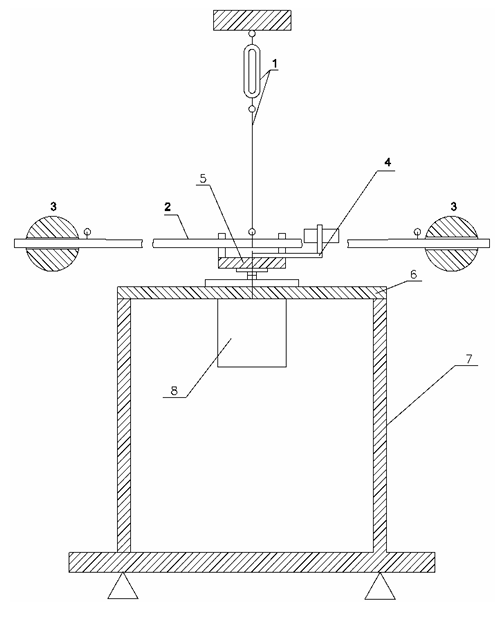
\includegraphics[scale=0.5]{stand} 
	}
	\legend{1 – система обезвешивания; 2 – штанга; 3 – груз; 4 – датчик угловой скорости с кронштейном для установки; 5 – элемент для передачи момента на выходной вал; 6 – плита установочная; 7 – основание; 8 – объект контроля}
	\caption{Функциональная схема инерционного стенда}
	\label{fig:stand} 
\end{figure}

Конструктивно такой стенд представляет собой установку с приводом и имитатором нагрузки, повторяющим момент инерции антенны, и системой обезвешивания. Реактивный момент определяется по динамике вращения выходного вала на основе зависимости

\begin{equation}
	\label{eq:eq_M_disturb}
	M=J_{\text{н}}\cdot \frac{d\omega}{dt}
\end{equation}

где \(J_{\text{н}}\) "--- момент инерции имитируемой нагрузки, \(\omega\) "--- угловая скорость.

Таким образом, метод сводиться к регистрации динамики вращения исполнительного механизма и последующему вычислению возмущающего момента через известные параметры имитируемой нагрузки.

Несмотря на практическую ценность, данный метод имеет ряд ограничений: использование имитатора вместо реальной нагрузки, необходимость изготовления отдельных моделей для каждого объекта, локальный характер измерений, а также невозможность анализа ситуаций с одновременной работой компенсирующих устройств. Эти недостатки не позволяют применить его для задач, связанных с оценкой реактивного момента в высокоточных оптико-электронных системах.


\underline{\textbf{Вторая глава}} анализу влияния алгоритма управления приводами  на величину некомпенсированных реактивных моментов при перенацеливании.

Рассматриваются три объекта: модуль направленного обзора с кардановым подвесом (две степени свободы), оптико-механическое устройство «Зеркало» с редукторными приводами по осям $OY$ и $OZ$, а также оптико-механический сканер для работы в режиме ВЗН. Во первых двух устройствах компенсация реактивного момента реализуется контрвращением маховика, кинематически жёстко связанного с приводом; редукторная связь уменьшает требуемый момент инерции маховика пропорционально $i^2$, что позволяет снизить массу и энергоёмкость узла при сохранении компенсирующего воздействия. В сканере компенсация осуществляется отдельным приводом. Такая архитектура позволяет независимо настраивать закон движения зеркала и компенсатора, оптимизируя спектр возмущений и синхронизацию с режимом ВЗН.

Рассмотрим результат воздействия реактивных моментов на основание с учётом расположения центра вращения карданова подвеса МНО относительно центра тяжести КА (Рисунок~\cref{fig:tikz_YPK})
\begin{figure}[h!]
	\centerfloat{
		\ifdefmacro{\tikzsetnextfilename}{\tikzsetnextfilename{tikz_example_compiled}}{}% присваиваемое предкомпилированному pdf имя файла (не обязательно)
		\resizebox{0.7\linewidth}{!}{%
		
	\begin{tikzpicture}[scale=1.6, >=stealth, font=\small]
		%X0Y0Z0 axis
		\draw [->, very thick] (13.75,13.25) -- (13.75,16.25)node[above] {$Y_0$};
		\draw [->, very thick] (13.75,13.25) -- (11.5,11.5) node[above] {$X_0$};
		\draw [->,very thick] (13.75,13.25) -- (11.25,13.75) node[above] {$Z_0$};
		\node at (13.85, 13.15) {$0_0$};
		%Z0 line
		\draw [thin, short] (11.25,13.75) -- (16.25,12.75);
		%Z line
		\draw [thin, short] (13.75,13.25) -- (16.75,13);
		
		%X0Y0Z0 axis proection
		\draw [thin] (10,8.25) -- (10,10.75) node[above] {$Y_0$};
		\draw [thin] (10,8.25) -- (7.5,8.75) node[above] {$Z_0$};
		\draw [thin] (10,8.25) -- (7.5,6.5) node[above] {$X_0$};
		
		
		%proection Z0 line
		\draw [thin, short] (7.5,8.75) -- (12.5,7.75);
		\draw [line width=0.9pt, ->,] (10,8.25) -- (10,10) node[right] {$Mda$};
		%OXYZ axis
		\draw [ ->, very thick] (10,8.25) -- (9.75,6.25) node[left] {$X$};
		\draw [->, very thick] (10,8.25) -- (9.32, 10.2) node[above] {$Y$};
		\draw[thick,->] (10, 10) arc[start angle=5,end angle=175,x radius=0.3cm, y radius=0.2cm];
		\node at (9.7, 10.3) {$\beta$};
		\draw [ ->, very thick] (10,8.25) -- (7,8.5) node[above] {$Z$};
		\node at (10.15,8.35) {$0$};
		\draw[thick,->] (8.8,8.5) arc[start angle=0,end angle=85,radius=-1.2cm];
		\node at (9.5, 7.5) {$\alpha$};
		%red line
		\draw [ color={rgb,255:red,245; green,0; blue,0}, line width=1.6pt, short] (13.75,13.25) -- (10,8.25);
		\node at (11, 10)[text=red] {$R$};
		\draw [ color=red, line width=0.2pt, ->,] (10,8.25) -- (9.75,9)node[left] {$Fb$};
		
		
		
		\draw [line width=0.9pt, ->,] (10,8.25) -- (7.8,8.43) node[above] {$Mdb$};
		\draw [ color=red, line width=0.2pt, ->,] (10,8.25) -- (8.5,8.37) node[above] {$Fa$};
		%blue circle
		\draw [ color={rgb,255:red,4; green,45; blue,251} , fill={rgb,255:red,45; green,166; blue,240}, line width=0.2pt ] (9.83,7) circle (0.25cm);
		
		
		
		\draw [ color=blue, very thick, short] (10,8.25) -- (9.83,7);
		\node at (10, 7.5)[text=blue] {$r$};
		\end{tikzpicture}
	}
		
	}
	\legend{}
	\caption[Пример \texttt{tikz} схемы]{Смещение центра масс блока зеркал МНО}\label{fig:tikz_YPK}
\end{figure}

Математическое описание реактивных моментов учитывает смещение центра масс зеркального блока относительно карданова подвеса на расстояние $r$ и несоосность центра подвеса с центром масс КА $(R_x,R_y,R_z)$. При работе приводов формируются моменты $M_{da}, M_{db}$ и реакции маховиков $M_{ma}, M_{mb}$. Результирующие моменты на осях кардана можно записать в виде:
\begin{equation}
	M_{ra} = F_a r + M_{da} - M_{ma}, 
	\qquad 
	M_{rb} = F_b r + M_{db} - M_{mb},
\end{equation}
где $F_a, F_b$ --- силы, действующие на узел зеркал. 

Силы, приложенные к подвесу, проецируются на оси $O_0X_0Y_0Z_0$, после чего суммарные моменты относительно центра масс КА имеют вид:
\begin{equation}
	\begin{aligned}
		M_{X_0} &= F_{Z_0}R_Y + F_{Y_0}R_Z + (M_{da}-M_{ma})\sin\alpha, \\
		M_{Y_0} &= F_{X_0}R_Z + F_{Z_0}R_X + (M_{da}-M_{ma}), \\
		M_{Z_0} &= F_{Y_0}R_X + (M_{db}-M_{mb})\cos\alpha.
	\end{aligned}
\end{equation}

Таким образом, результирующие реактивные моменты представляют собой сумму двух составляющих: 
\begin{itemize}
	\item моментов, вызванных смещением центра карданова подвеса относительно центра масс КА ($R_x, R_y, R_z$);
	\item остаточных моментов, возникающих из-за неполной компенсации приводами маховиков.
\end{itemize}


Отдельное внимание уделяется влиянию профиля разгона привода на спектр возмущающих воздействий. Трапецеидальный закон прост и время-оптимален при заданных ограничениях на $\alpha$ и $\omega$, но содержит скачки ускорения (рывок), что порождает широкополосные гармоники. Синусоидальный профиль обеспечивает непрерывность не только $\omega$ и $\alpha$, но и плавность изменений рывка. 
Для оценки оптимальности профиля используется критерий Рэлея, характеризующий отношение энергии рывка к энергии ускорения:

\begin{equation}
	\label{eq:relay}
	\mathcal{R}[\epsilon] =
	\frac{\displaystyle \int_{0}^{T} \bigl(\dot{\epsilon}(t)\bigr)^{2}\,dt}
	{\displaystyle \int_{0}^{T} \epsilon^{2}(t)\,dt},
\end{equation}

где $\epsilon(t)$ --- функция ускорения, $T$ --- длительность манёвра.

Минимальное значение функционала достигается для гармонического профиля ускорения, что можно показать разложением в ряд Фурье. 
При граничных условиях
\begin{equation}
	\epsilon(0) = \epsilon(T) = 0, 
	\qquad 
	\int_{0}^{T} \epsilon(t)\,dt = 0,
\end{equation}
первой допустимой собственной функцией является синус с удвоенной частотой, и оптимальный профиль имеет вид:
\begin{equation}
	\epsilon(t) = \epsilon_0 \sin\!\left(\frac{2\pi t}{T}\right).
\end{equation}

Таким образом, синусоидальный закон обеспечивает минимум функционала Рэлея, то есть наилучшее сглаживание ускорений и рывков. 
Его спектр ограничен одной гармоникой, что минимизирует возбуждение высокочастотных колебаний и снижает уровень микровибраций, передаваемых на основание космического аппарата.





\underline{\textbf{Третья глава}} посвящена разработке и созданию испытательного стенда для измерения остаточных реактивных моментов оптико-механических систем.

Теоретическая модель стенда задаётся как колебательное звено второго порядка:

\begin{equation}
	\label{eq:stadeq}
	J\cdot \frac{d^2\varphi}{dt^2}+b \cdot \frac{d\varphi}{dt}+ c \cdot \varphi = M(t)
\end{equation}

где \(J\) --- момент инерции рамы вместе с установленной оптической системой, \(\varphi\) --- угол поворота рамы относительно равновесного положения, \(b\) --- коэффициент затухания, \(с\) --- коэффициент крутильной жёсткости, \(M(t)\) --- реактивный момент.

Для корректного воспроизведения динамики необходимо, чтобы собственная частота маятника была смещена относительно диапазона характерных частот воздействия. В данном случае стенд спроектирован таким образом, что возмущающее воздействие проявляется в послерезонансной области. В этом случае колебательное звено работает как механический фильтр низких частот, подавляющий высокочастотные вибрации основания и внешние помехи, при этом сохраняется информативность основной составляющей измеряемого момента.

Моделирование стенда показало, что при увеличении декремента затухания выше $\xi=0,1$ форма выходного сигнала сильно искажается: снижается амплитуда и появляется фазовый сдвиг относительно входного воздействия. Поэтому при проектировании подвеса использовались материалы и схемы крепления, обеспечивающие малый уровень диссипативных потерь и обеспечивающие $\xi \leq 0,1$.



Измерительный стенд выполнен в виде подвесной системы, обеспечивающей исследуемой ОМС одну степень свободы. Подвижная часть состоит из рамы, подвешенной на двух струнах и способной поворачиваться вокруг вертикальной оси. Внутри рамы установлен жёсткий каркас с основанием для крепления ОМС. Конструкция предусматривает возможность поворота каркаса вокруг горизонтальной оси, что позволяет фиксировать ОМС в двух положениях — с осью $OY$ или $OZ$, совмещённой с направлением струн. Точная балансировка осуществляется с помощью грузов, устанавливаемых на пальцы каркаса.

Узел подвеса включает штабелёр, раму на проволочном подвесе, кантователь и балансировочные грузы. При подъёме рамы штабелёром подвес разарретируется и получает возможность свободного вращения на угол ±5° вокруг вертикальной оси. При опускании рама фиксируется и полностью исключает перемещения относительно основания.

Оптико-механическая система монтируется на посадочное место кантователя. Поворот кантователя вокруг горизонтальной оси позволяет выбрать направление оси поворота, совпадающей с вертикальной осью стенда. В процессе поворота подвижной части оптико-механической системы возникает реактивный момент, вызывающий вращение рамы вокруг вертикальной оси. Угловое движение регистрируется волоконно-оптическим гироскопом, установленным на подвесной раме. Дополнительно в состав установки включён тестовый маховик с известным моментом инерции, используемый для формирования контролируемого возмущающего момента. Совместное применение гироскопа и маховика обеспечивает как регистрацию угловых колебаний, так и калибровку чувствительности системы. Общий вид установки приведён на рисунке ~\cref{fig:yoiom}.

\begin{figure}[!h] 
	\centerfloat{
		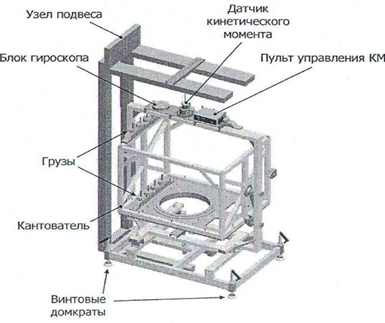
\includegraphics[scale=1]{yoim-cxem} 
	}
	\caption{Стенд измерения реактивного момента}
	\label{fig:yoiom} 
\end{figure}

Методика измерений основана на сравнении ускорений колебаний при эталонном и исследуемом воздействиях. Гироскоп регистрирует угловую скорость $\omega(t)$, угловое ускорение определяется численным дифференцированием:

\begin{equation}
	\label{eq:mean_acc}
	\varepsilon_{i}
	= \frac{\overline{\omega}_{i+1}-\overline{\omega}_{i}}{\Delta t},
	\qquad
	\Delta t = \frac{1}{f_s}.
\end{equation}

где $f_s$ --- частота дискретизации гироскопа,

Остаточный реактивный момент находится по соотношению
\begin{equation}
	M = M_m\frac{\varepsilon_o}{\varepsilon_m},
\end{equation}

где \(M_m = J_m\alpha_m\)"--- известный тестовый момент маховика, \(\varepsilon_o\)"--- ускорение рамы, вызванное поворотом подвижной части оптико-механической системы, \(\varepsilon_m\)"--- ускорение вызванное тестовым моментом.

Разработанный измерительный стенд прошёл метрологическую аттестацию
в установленном порядке. Аттестация выполнена в АО «НПО Техномаш»
им. С.~А.~Афанасьева при поддержке Госкорпорации «Роскосмос».
По результатам выдано свидетельство №~030-500/2024-61
(РОСС~RU.0001.310066/2024), запись в государственном реестре
ФР.1.28.2024.49055. Методика измерений признана соответствующей
ГОСТ~Р~8.563–2009. Диапазон измеряемых моментов составляет
от $10^{-3}$ до $1\,\text{Н}\cdot\text{м}$ при относительной
неопределённости порядка $1\,\%$, что подтверждает пригодность стенда
для поверочных работ и исследовательских испытаний оптико-механических систем.

\underline{\textbf{Четвертая главе}} посвящена экспериментальным исследованиям и проверке работоспособности разработанного стенда.

Для проверки достоверности методики выполнена серия измерений реактивного момента модуля направленного обзора.
В качестве опорного воздействия использовался момент $M_{\text{тест}}=\SI{0.005}{\newton\meter}$;
регистрировалась угловая скорость колебаний, затем выполнялось усреднение по нескольким измерениям и численное дифференцирование (рис.~\cref{fig:test-gyro-acc}).

\begin{figure}[h!]
	\centering
	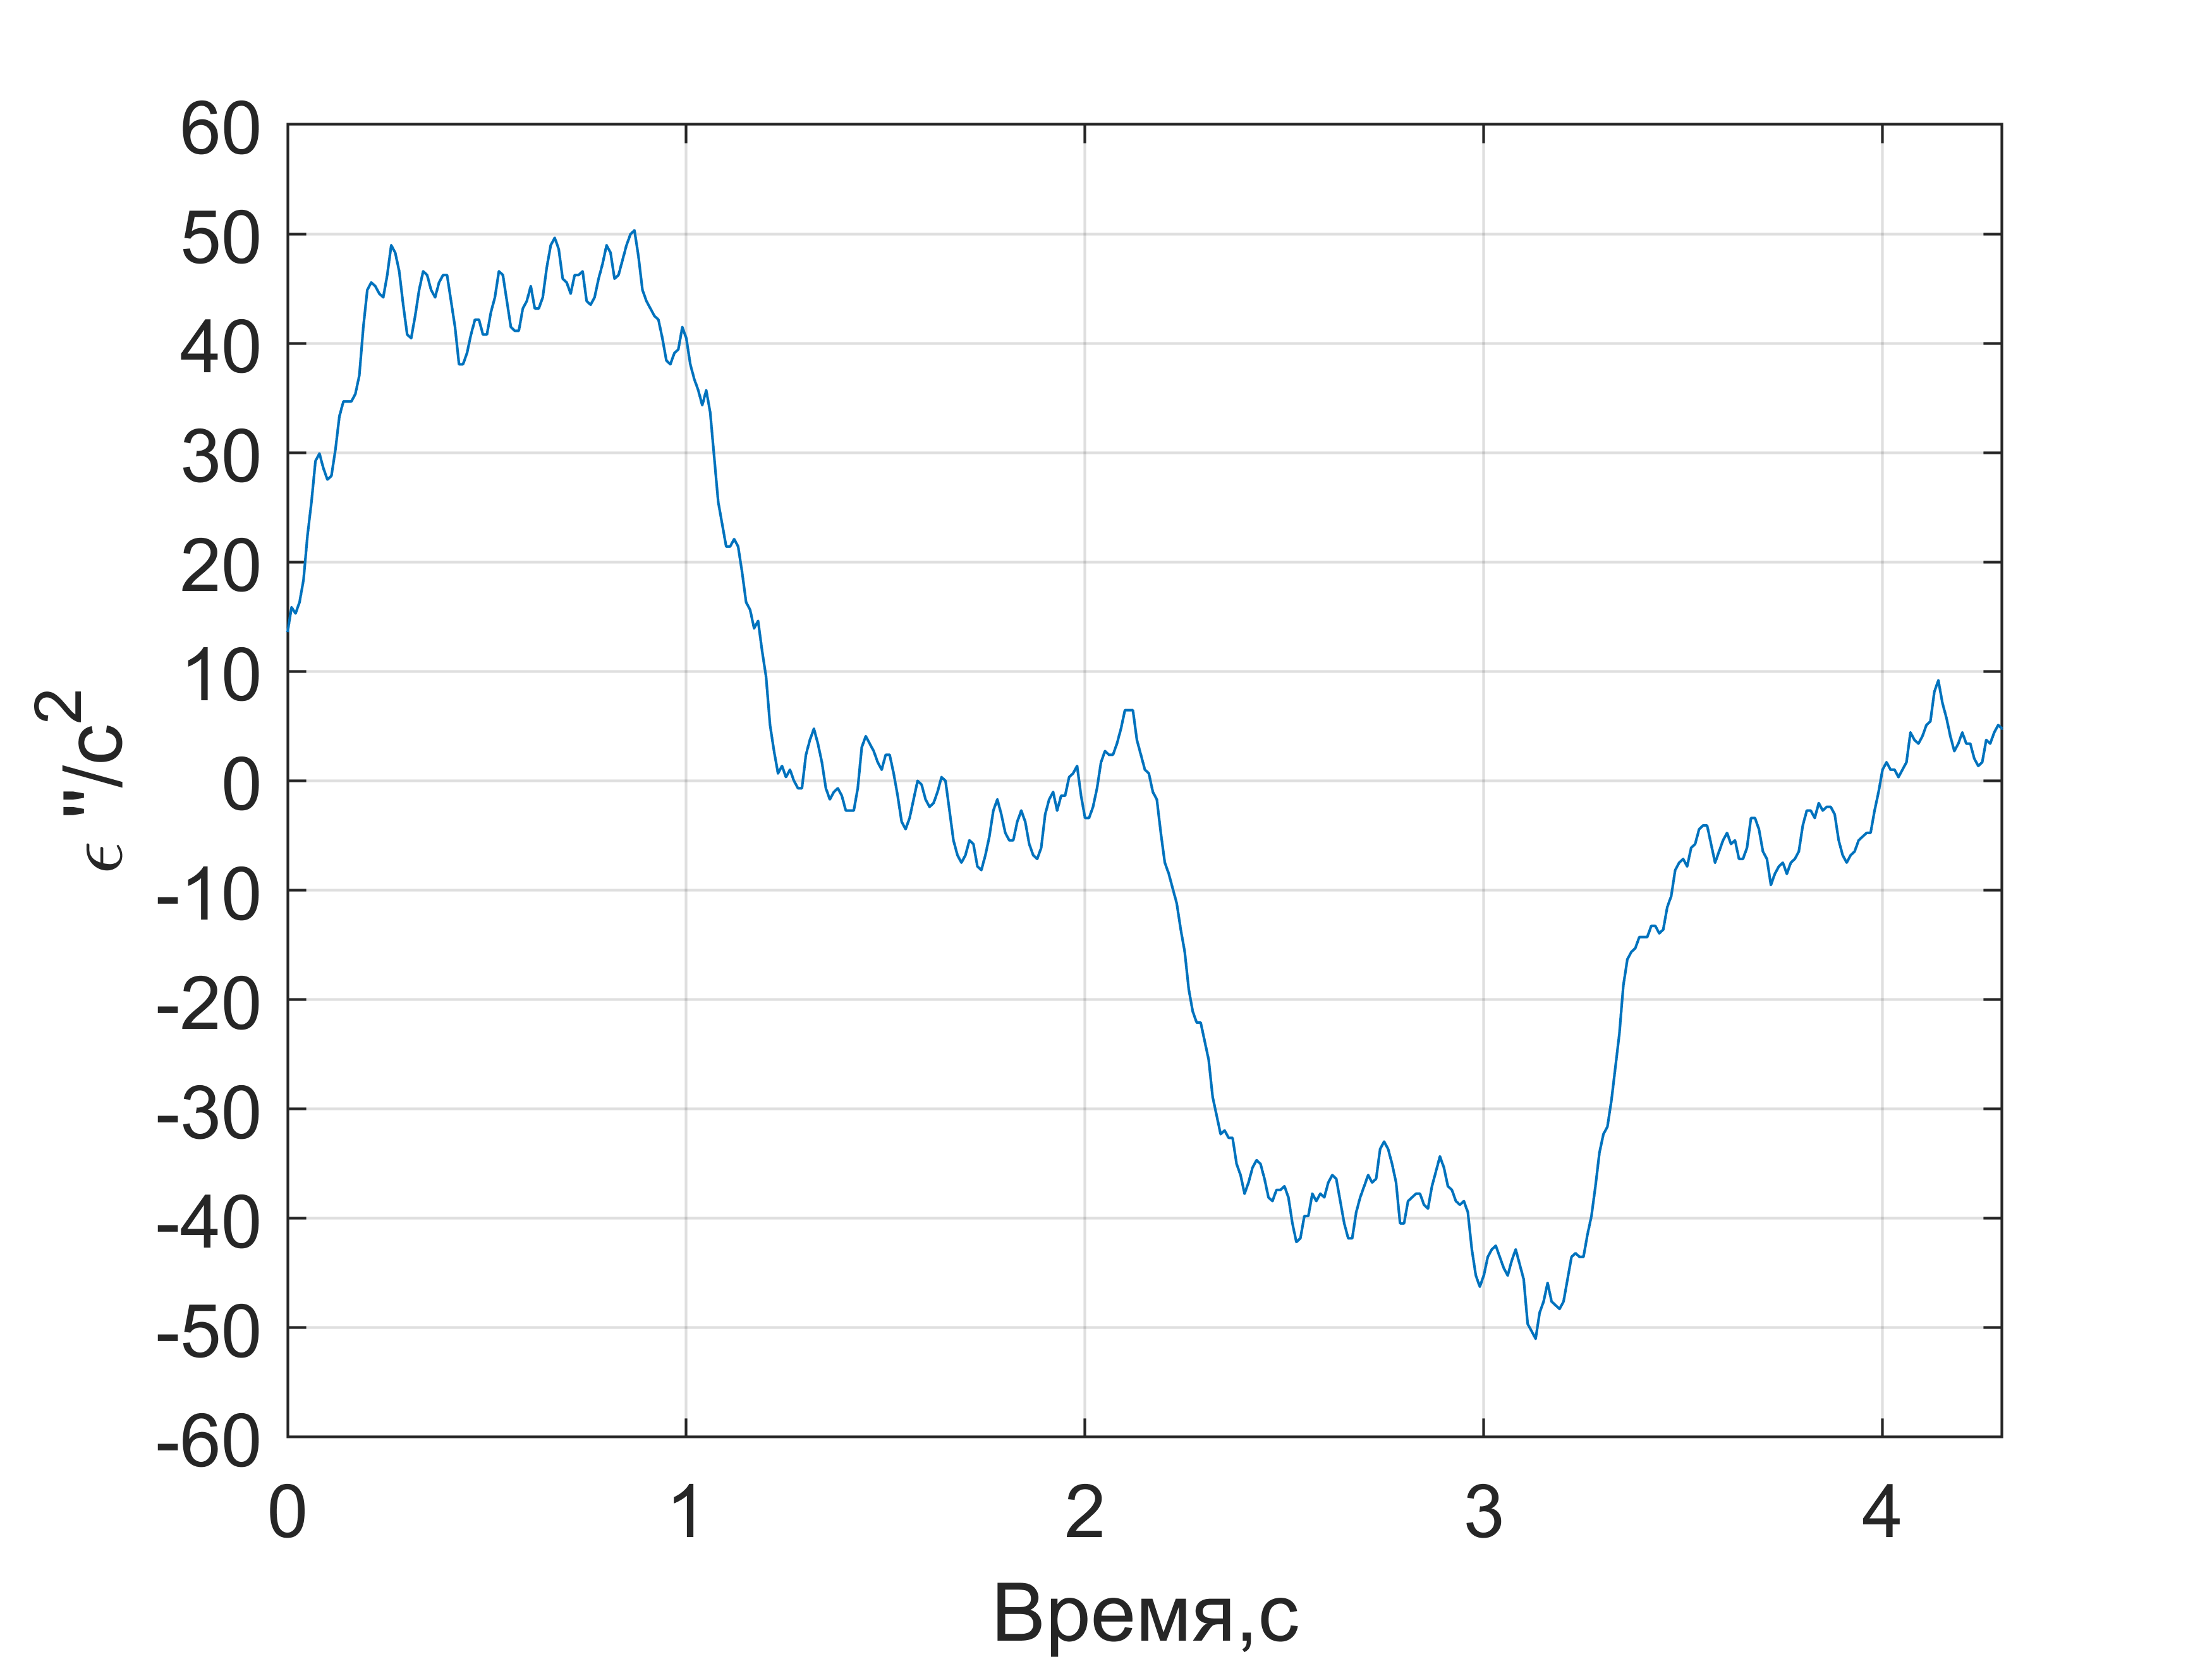
\includegraphics[scale=0.3]{matlab/img/test-gyro-acc}
	\caption{Ускорение при тестовом воздействии}
	\label{fig:test-gyro-acc}
\end{figure}

Затем выполнены повороты МНО вокруг осей $OZ$ и $OY$ (по 10 реализаций), обработка проводилась аналогично:
усреднение по ансамблю, дифференцирование
(рис.~\cref{fig:oz-gyro}).

\begin{figure}[!h]
	\begin{minipage}[b]{0.49\linewidth}\centering
		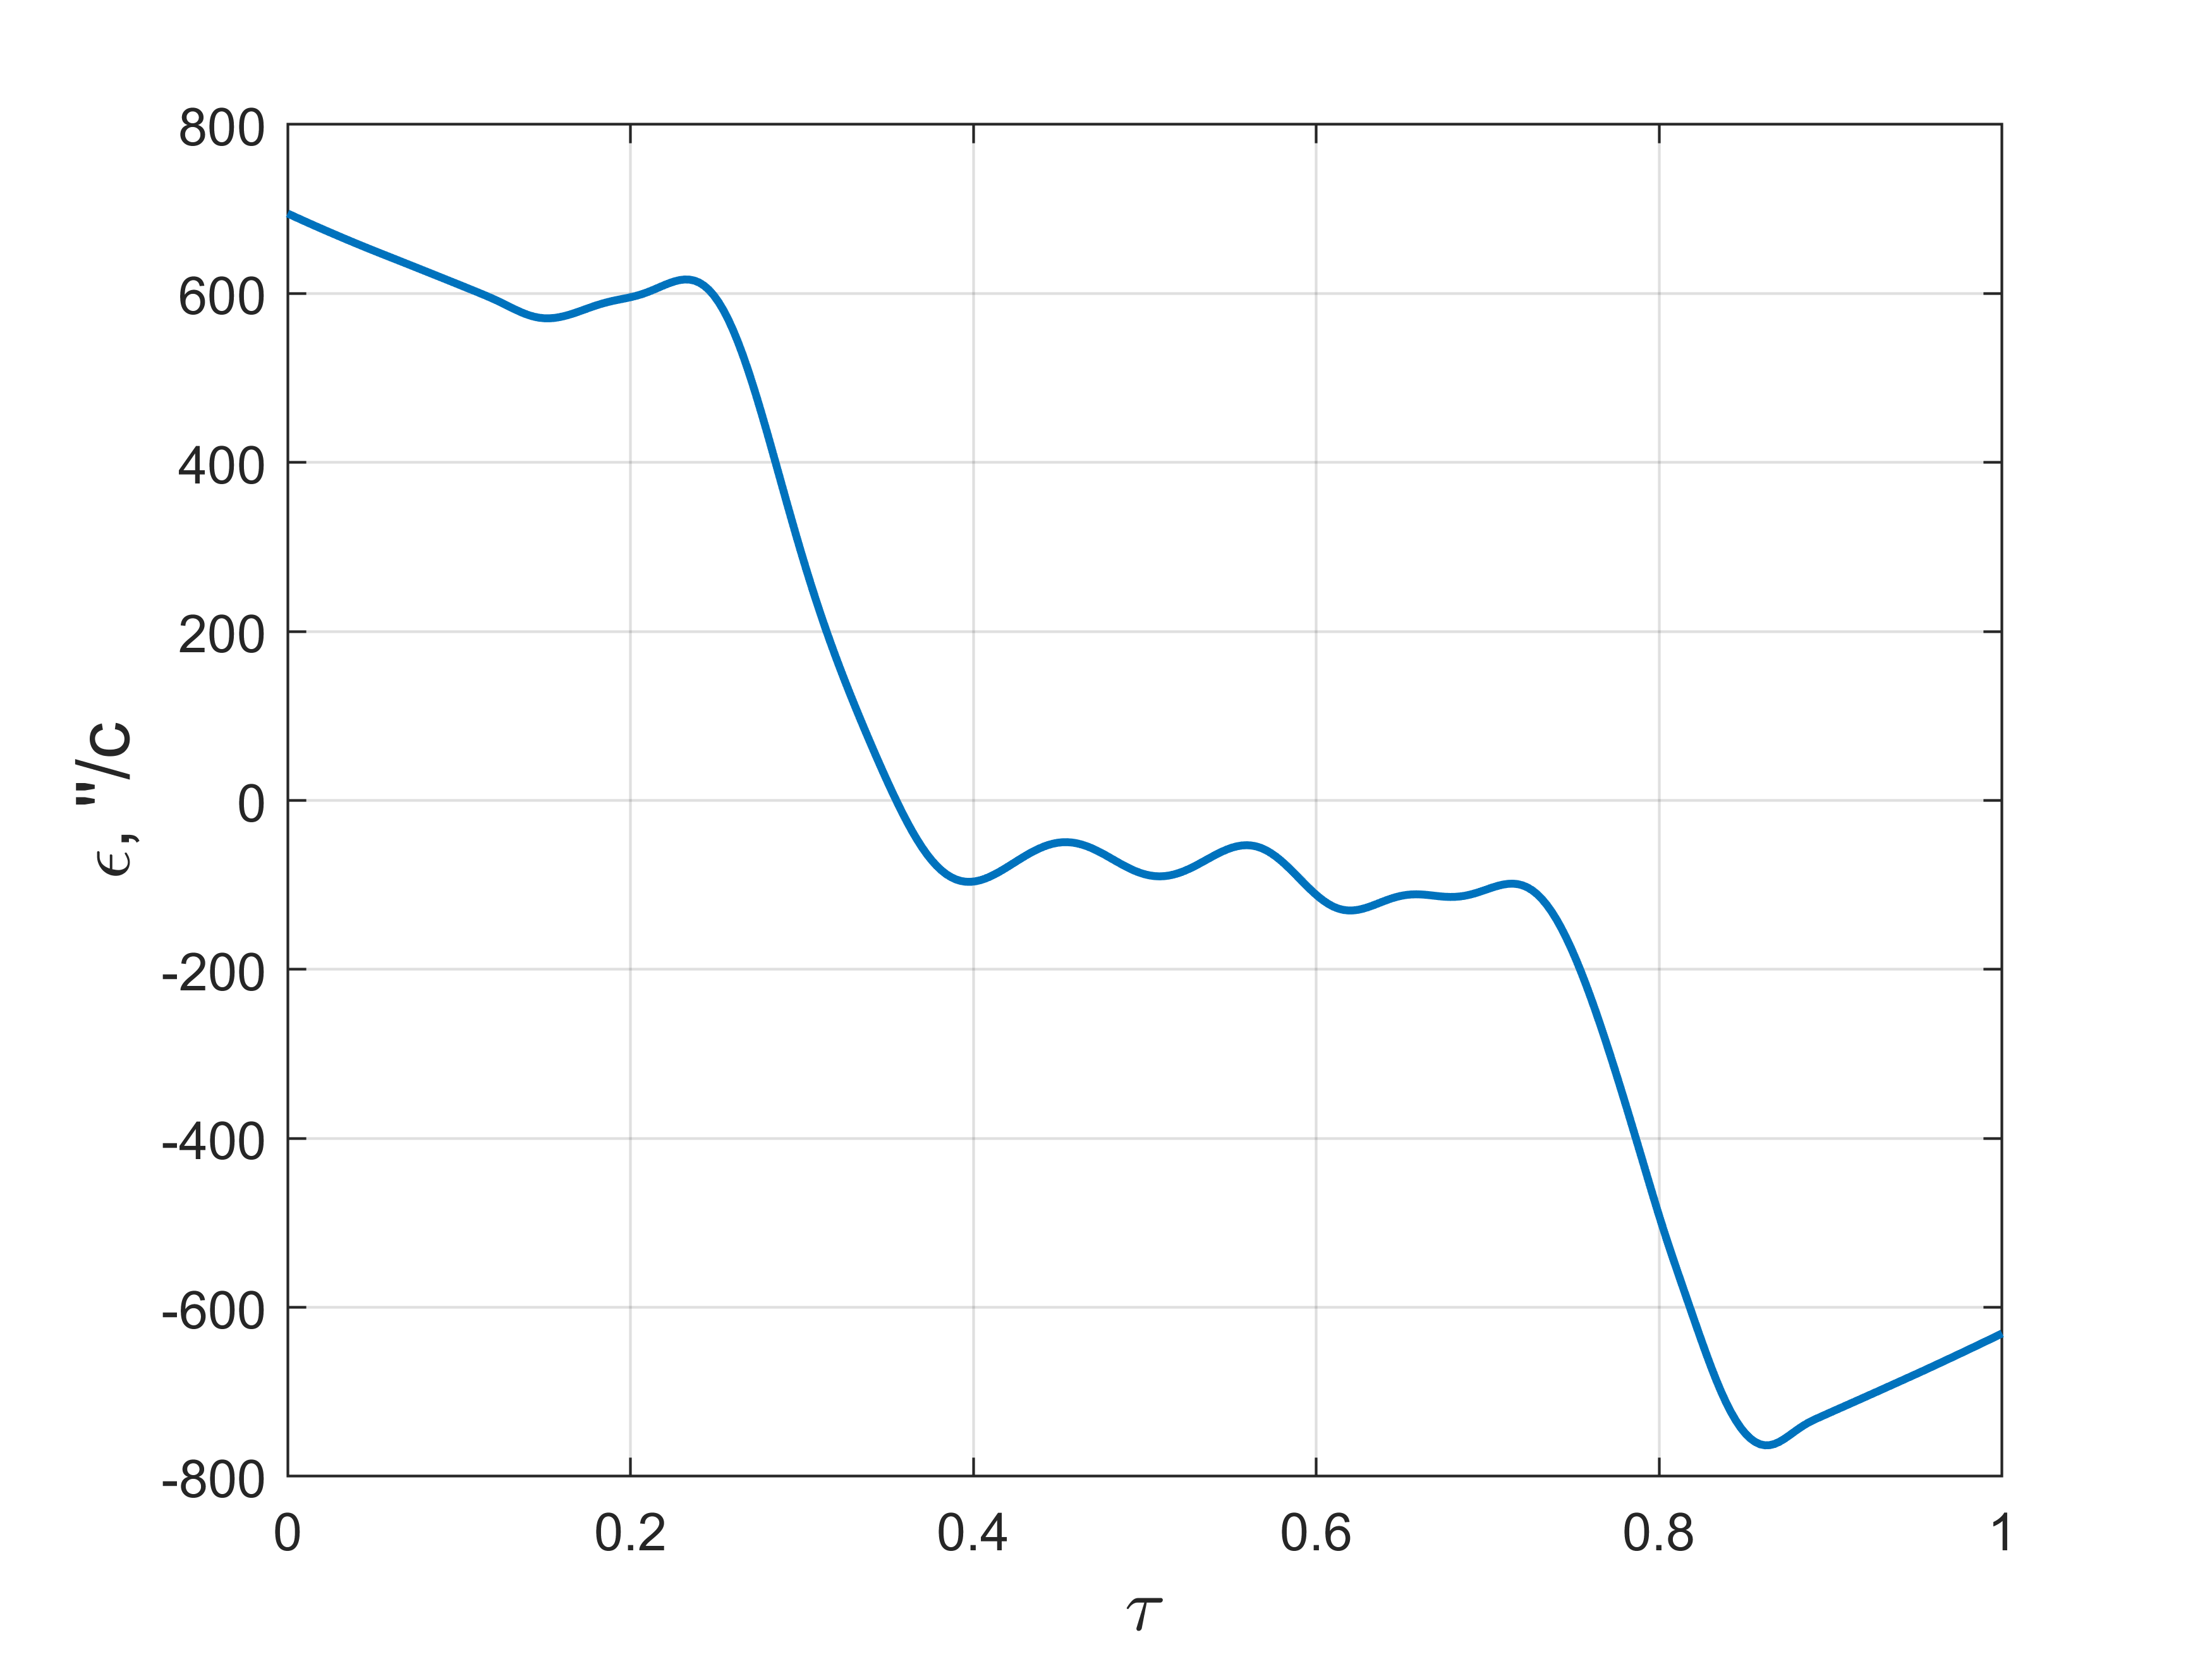
\includegraphics[width=0.8\linewidth]{matlab/img/oy-gyro-acc.png}\\[-2pt] a)
	\end{minipage}
	\hfill
	\begin{minipage}[b]{0.49\linewidth}\centering
		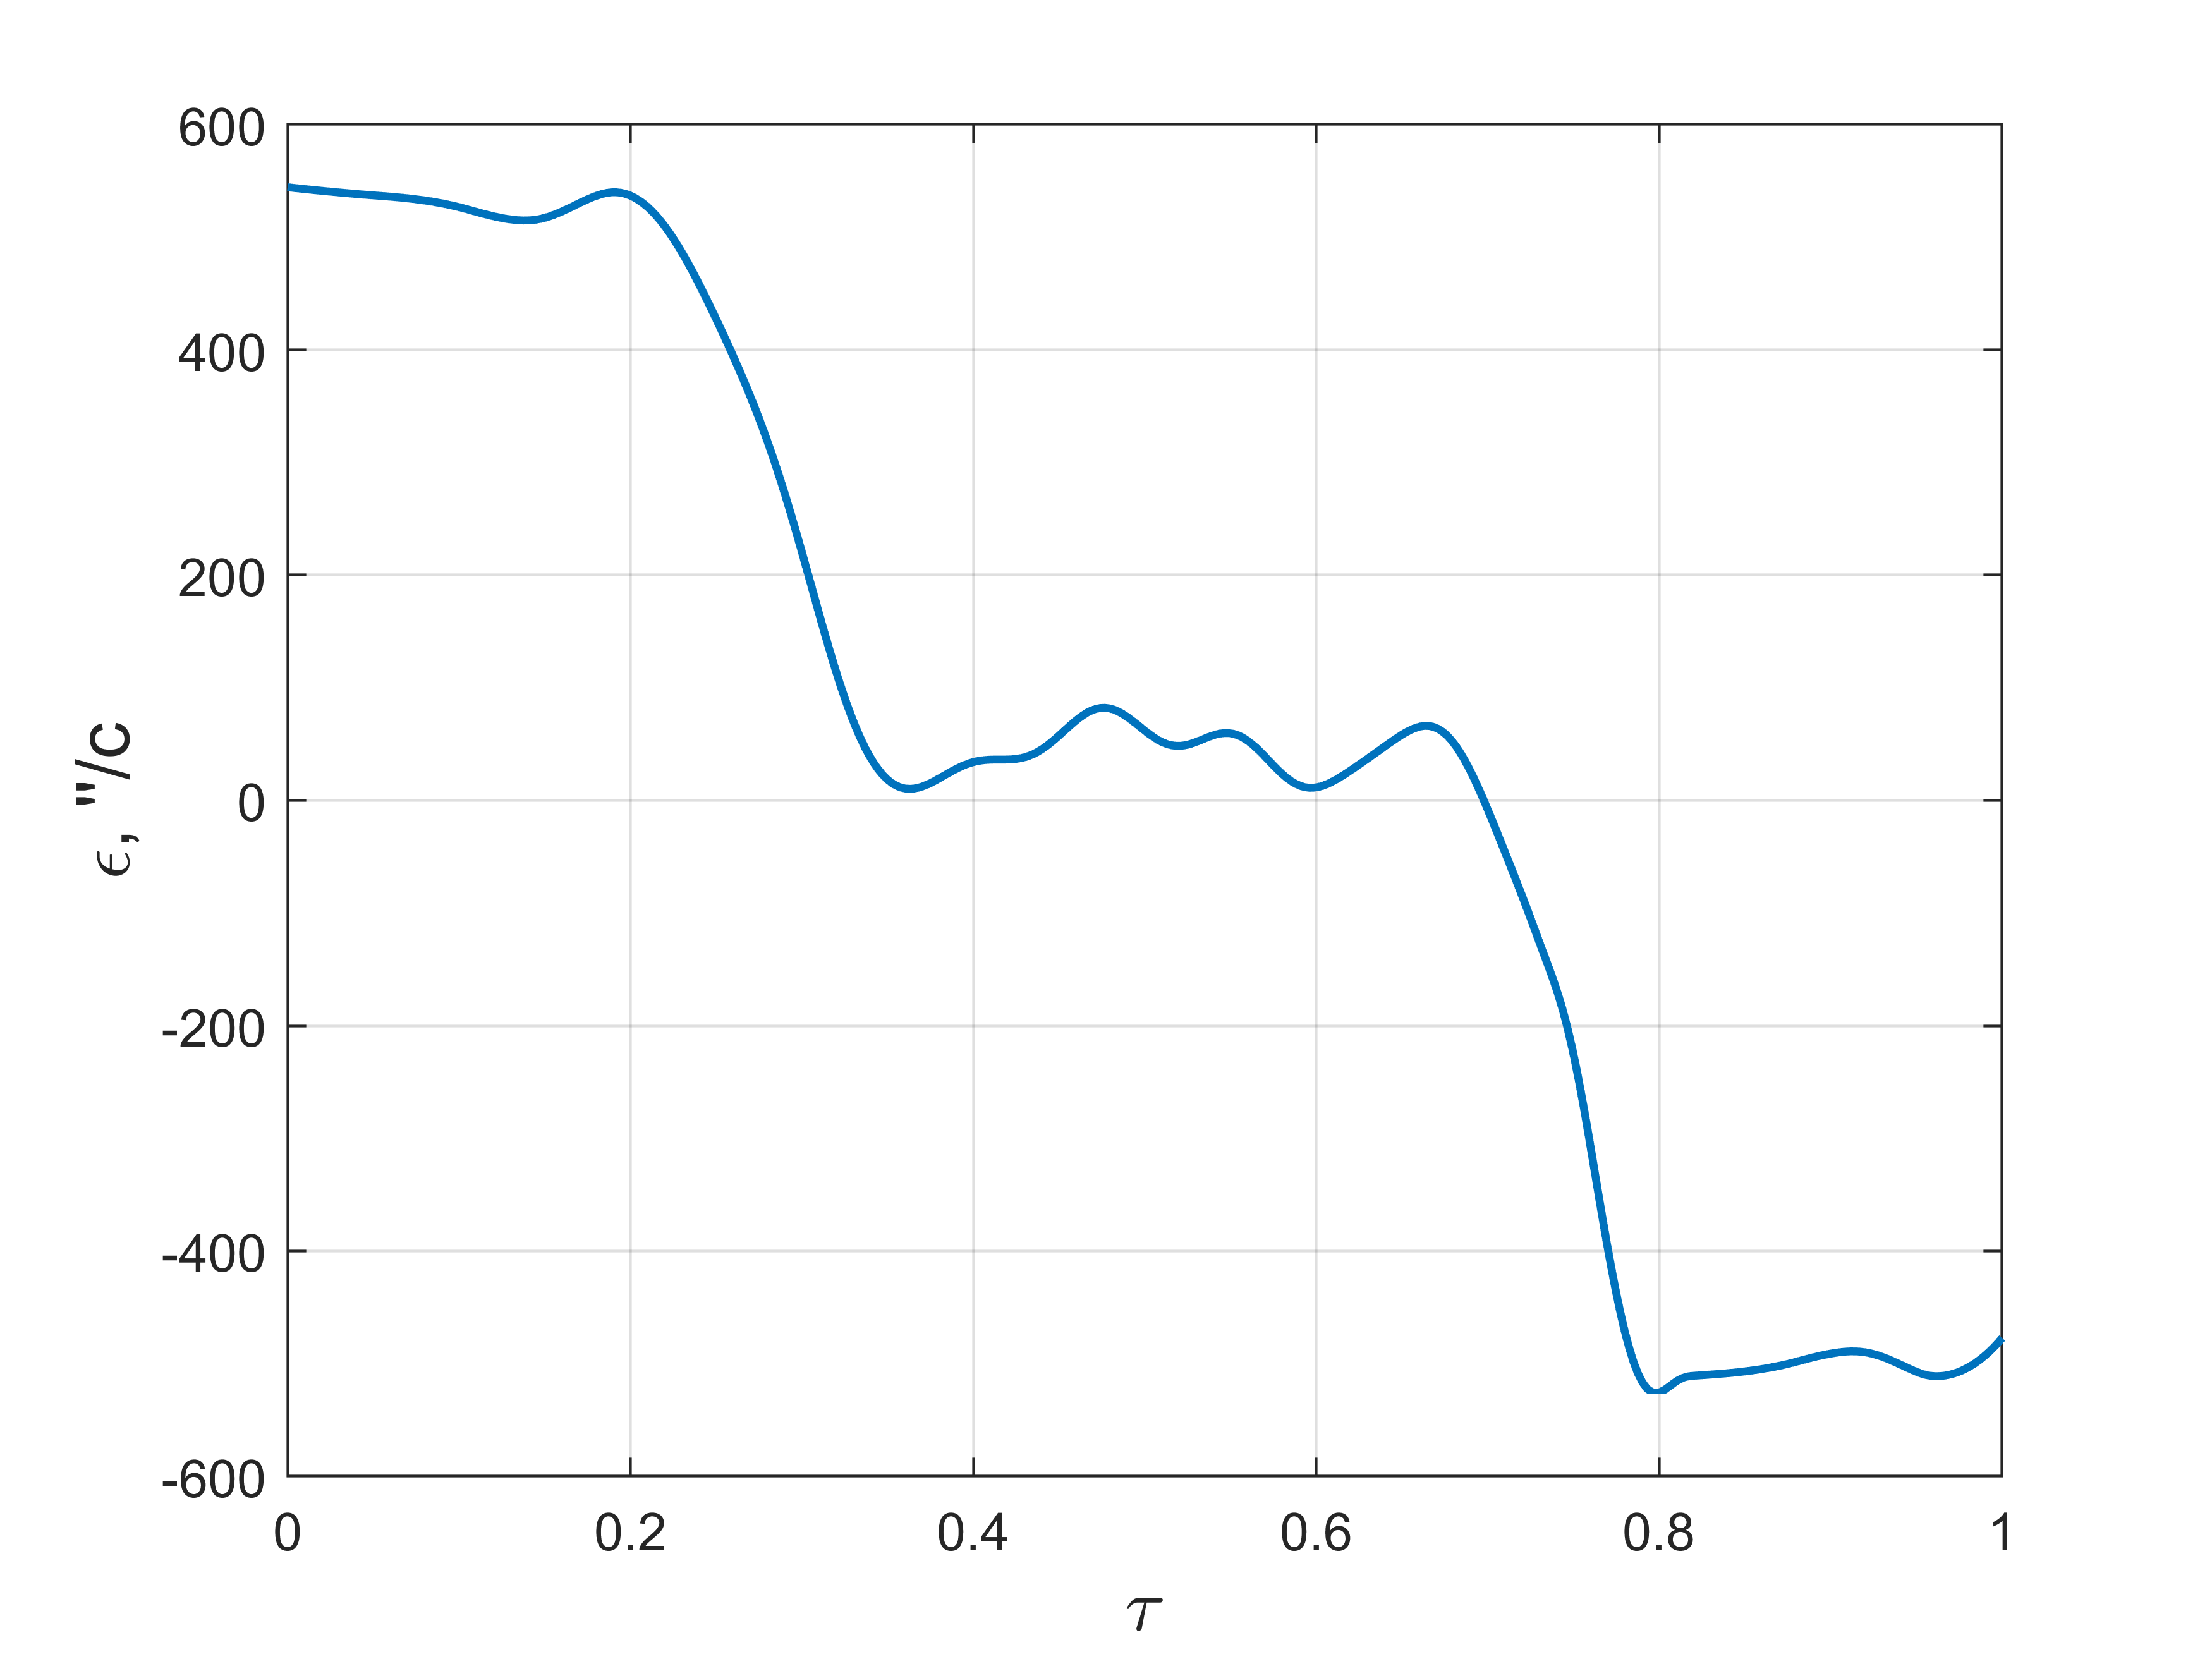
\includegraphics[width=0.8\linewidth]{matlab/img/oz-gyro-acc.png}\\[-2pt] б)
	\end{minipage}
	\caption{Ускорение рамы при поворот МНО вокруг a) $OY$ б) $OZ$}
	\label{fig:oz-gyro}
\end{figure}

Остаточный момент МНО определялся сравнением с эталоном:
\[
M_{\text{МНО}} = M_{\text{тест}}\cdot\frac{\varepsilon_{\text{МНО}}}{\varepsilon_{\text{тест}}}\!,
\]

По результатам обработки экспериментальных данных величина реактивного момента составила $M_y = \SI{0,076}{\newton\meter}$ при повороте вокруг оси $Y$ и $M_z = \SI{0,055}{\newton\meter}$ при повороте вокруг оси $Z$ (см. рис.~\cref{fig:omn-mom}).

\begin{figure}[!h]
	\begin{minipage}[b]{0.49\linewidth}\centering
		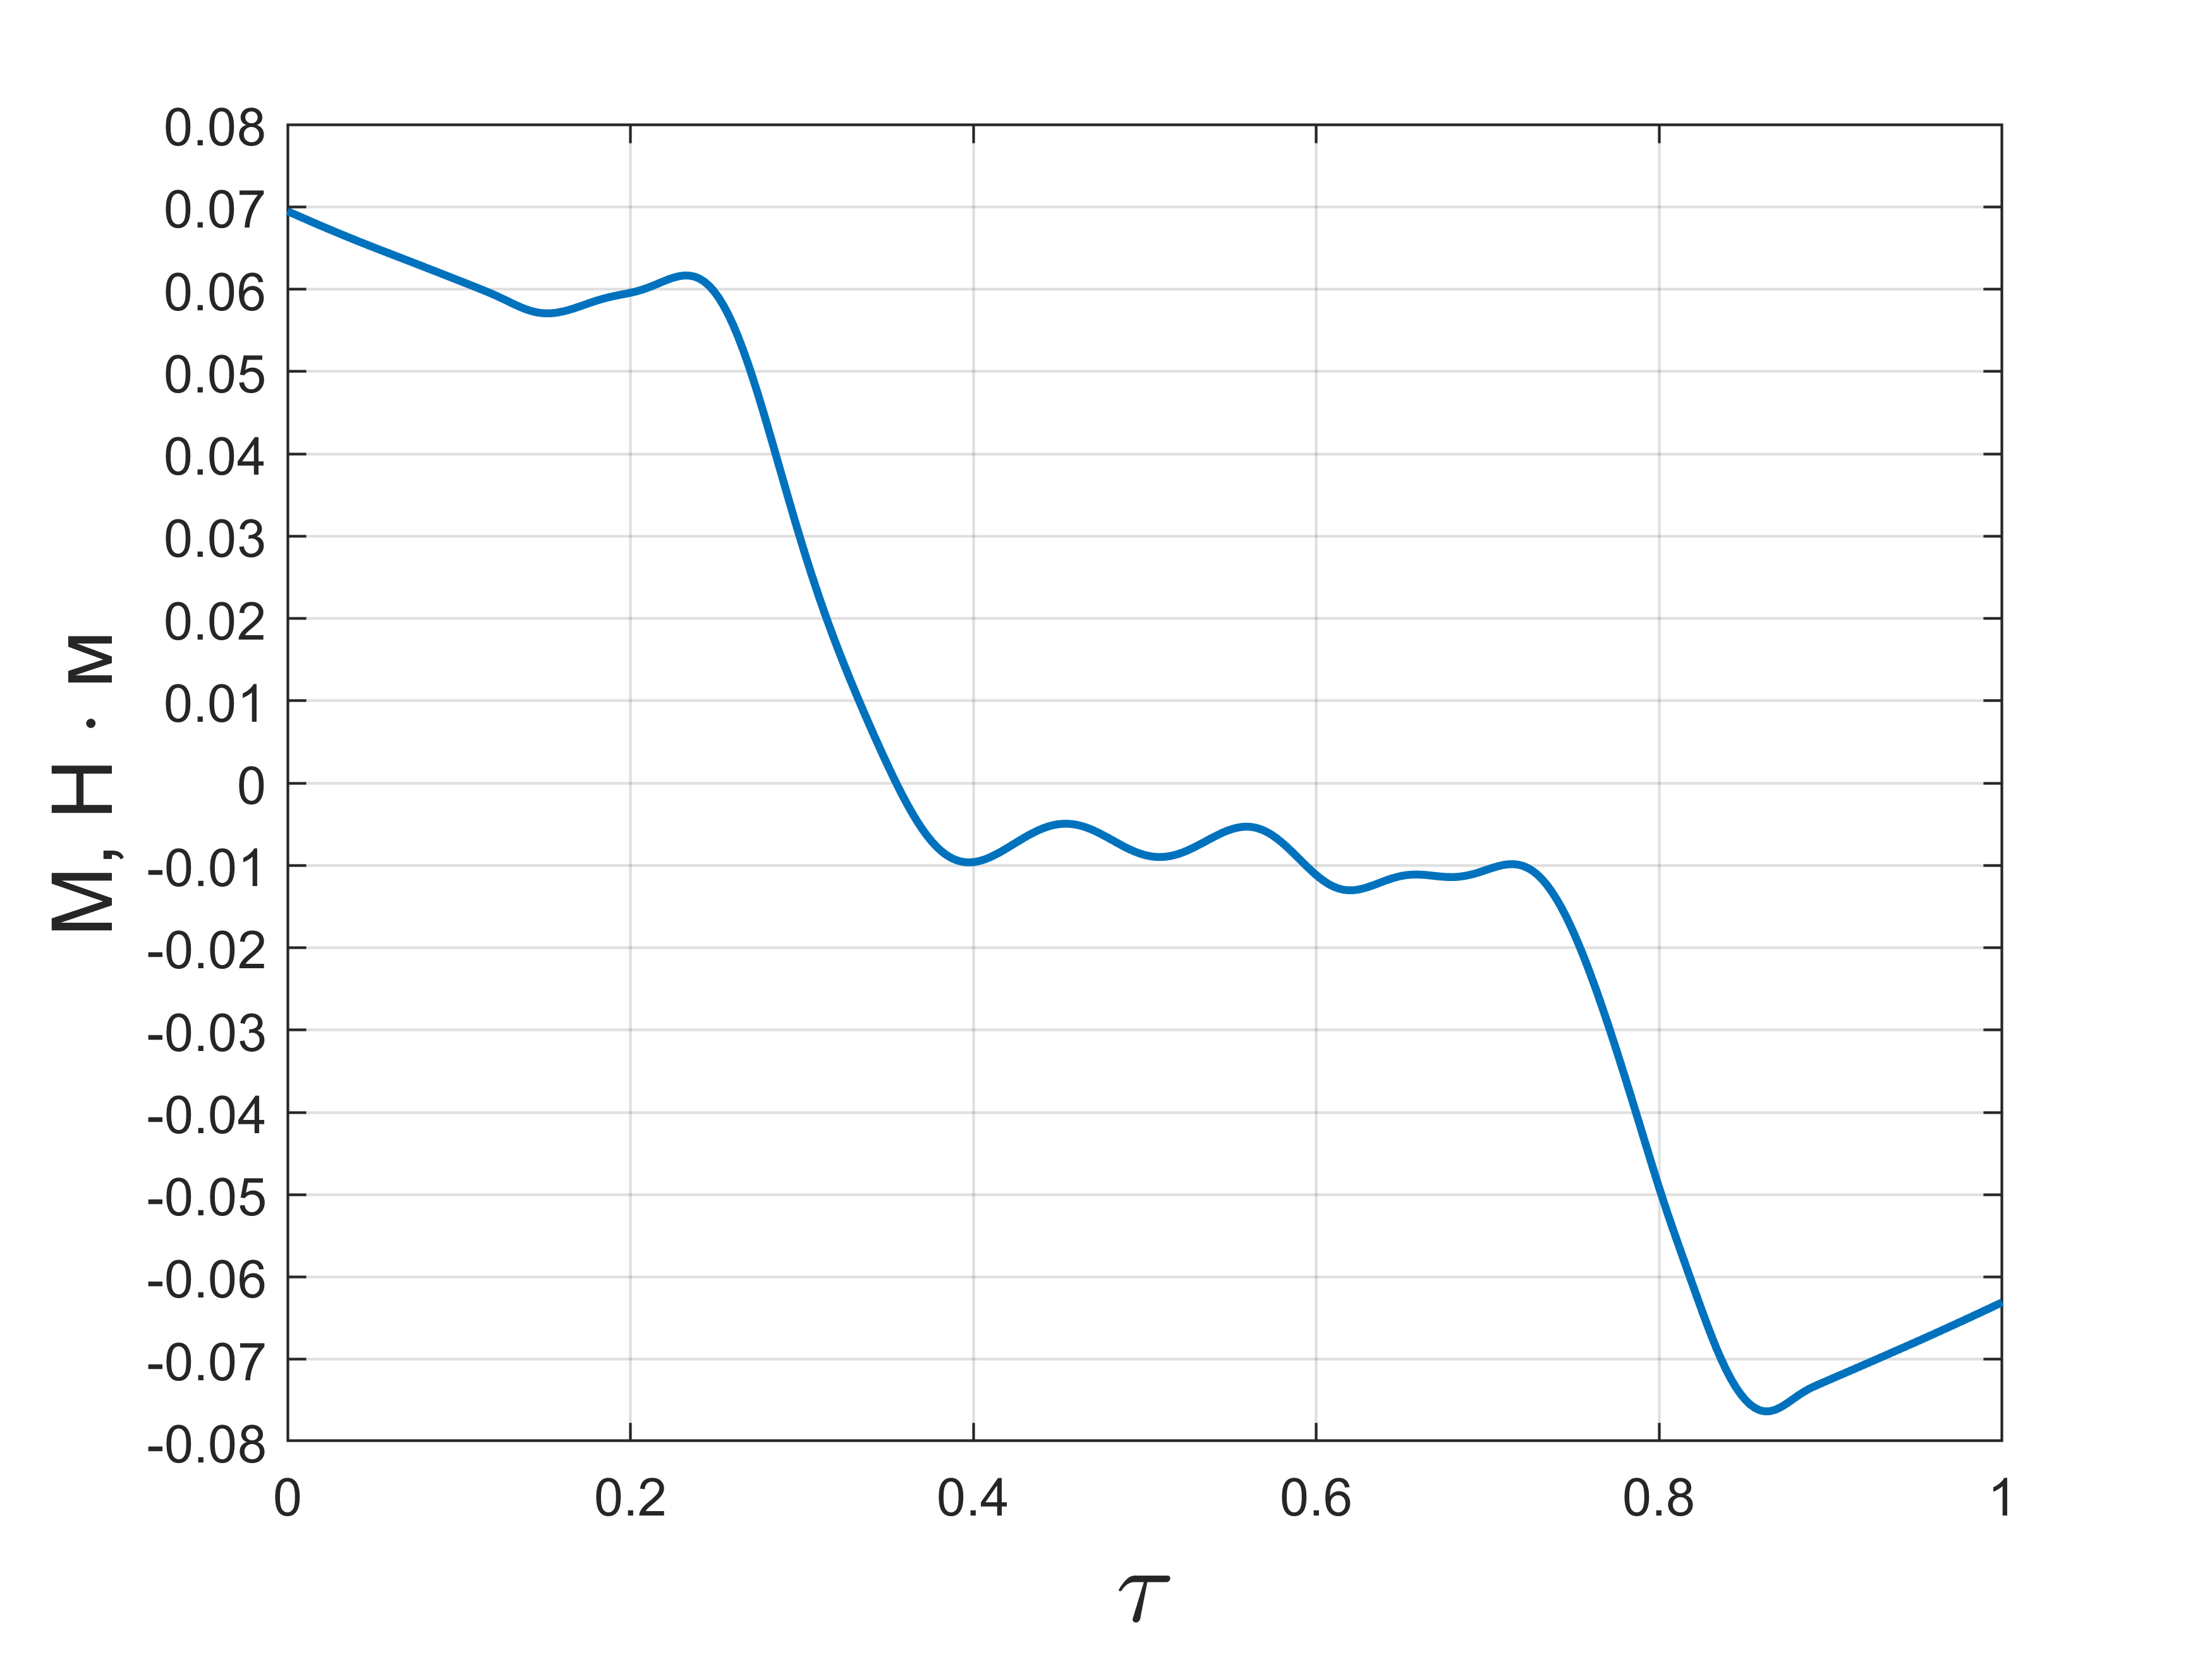
\includegraphics[width=0.8\linewidth]{matlab/img/oy-gyro-mom.png}\\[-2pt] a)
	\end{minipage}
	\hfill
	\begin{minipage}[b]{0.49\linewidth}\centering
		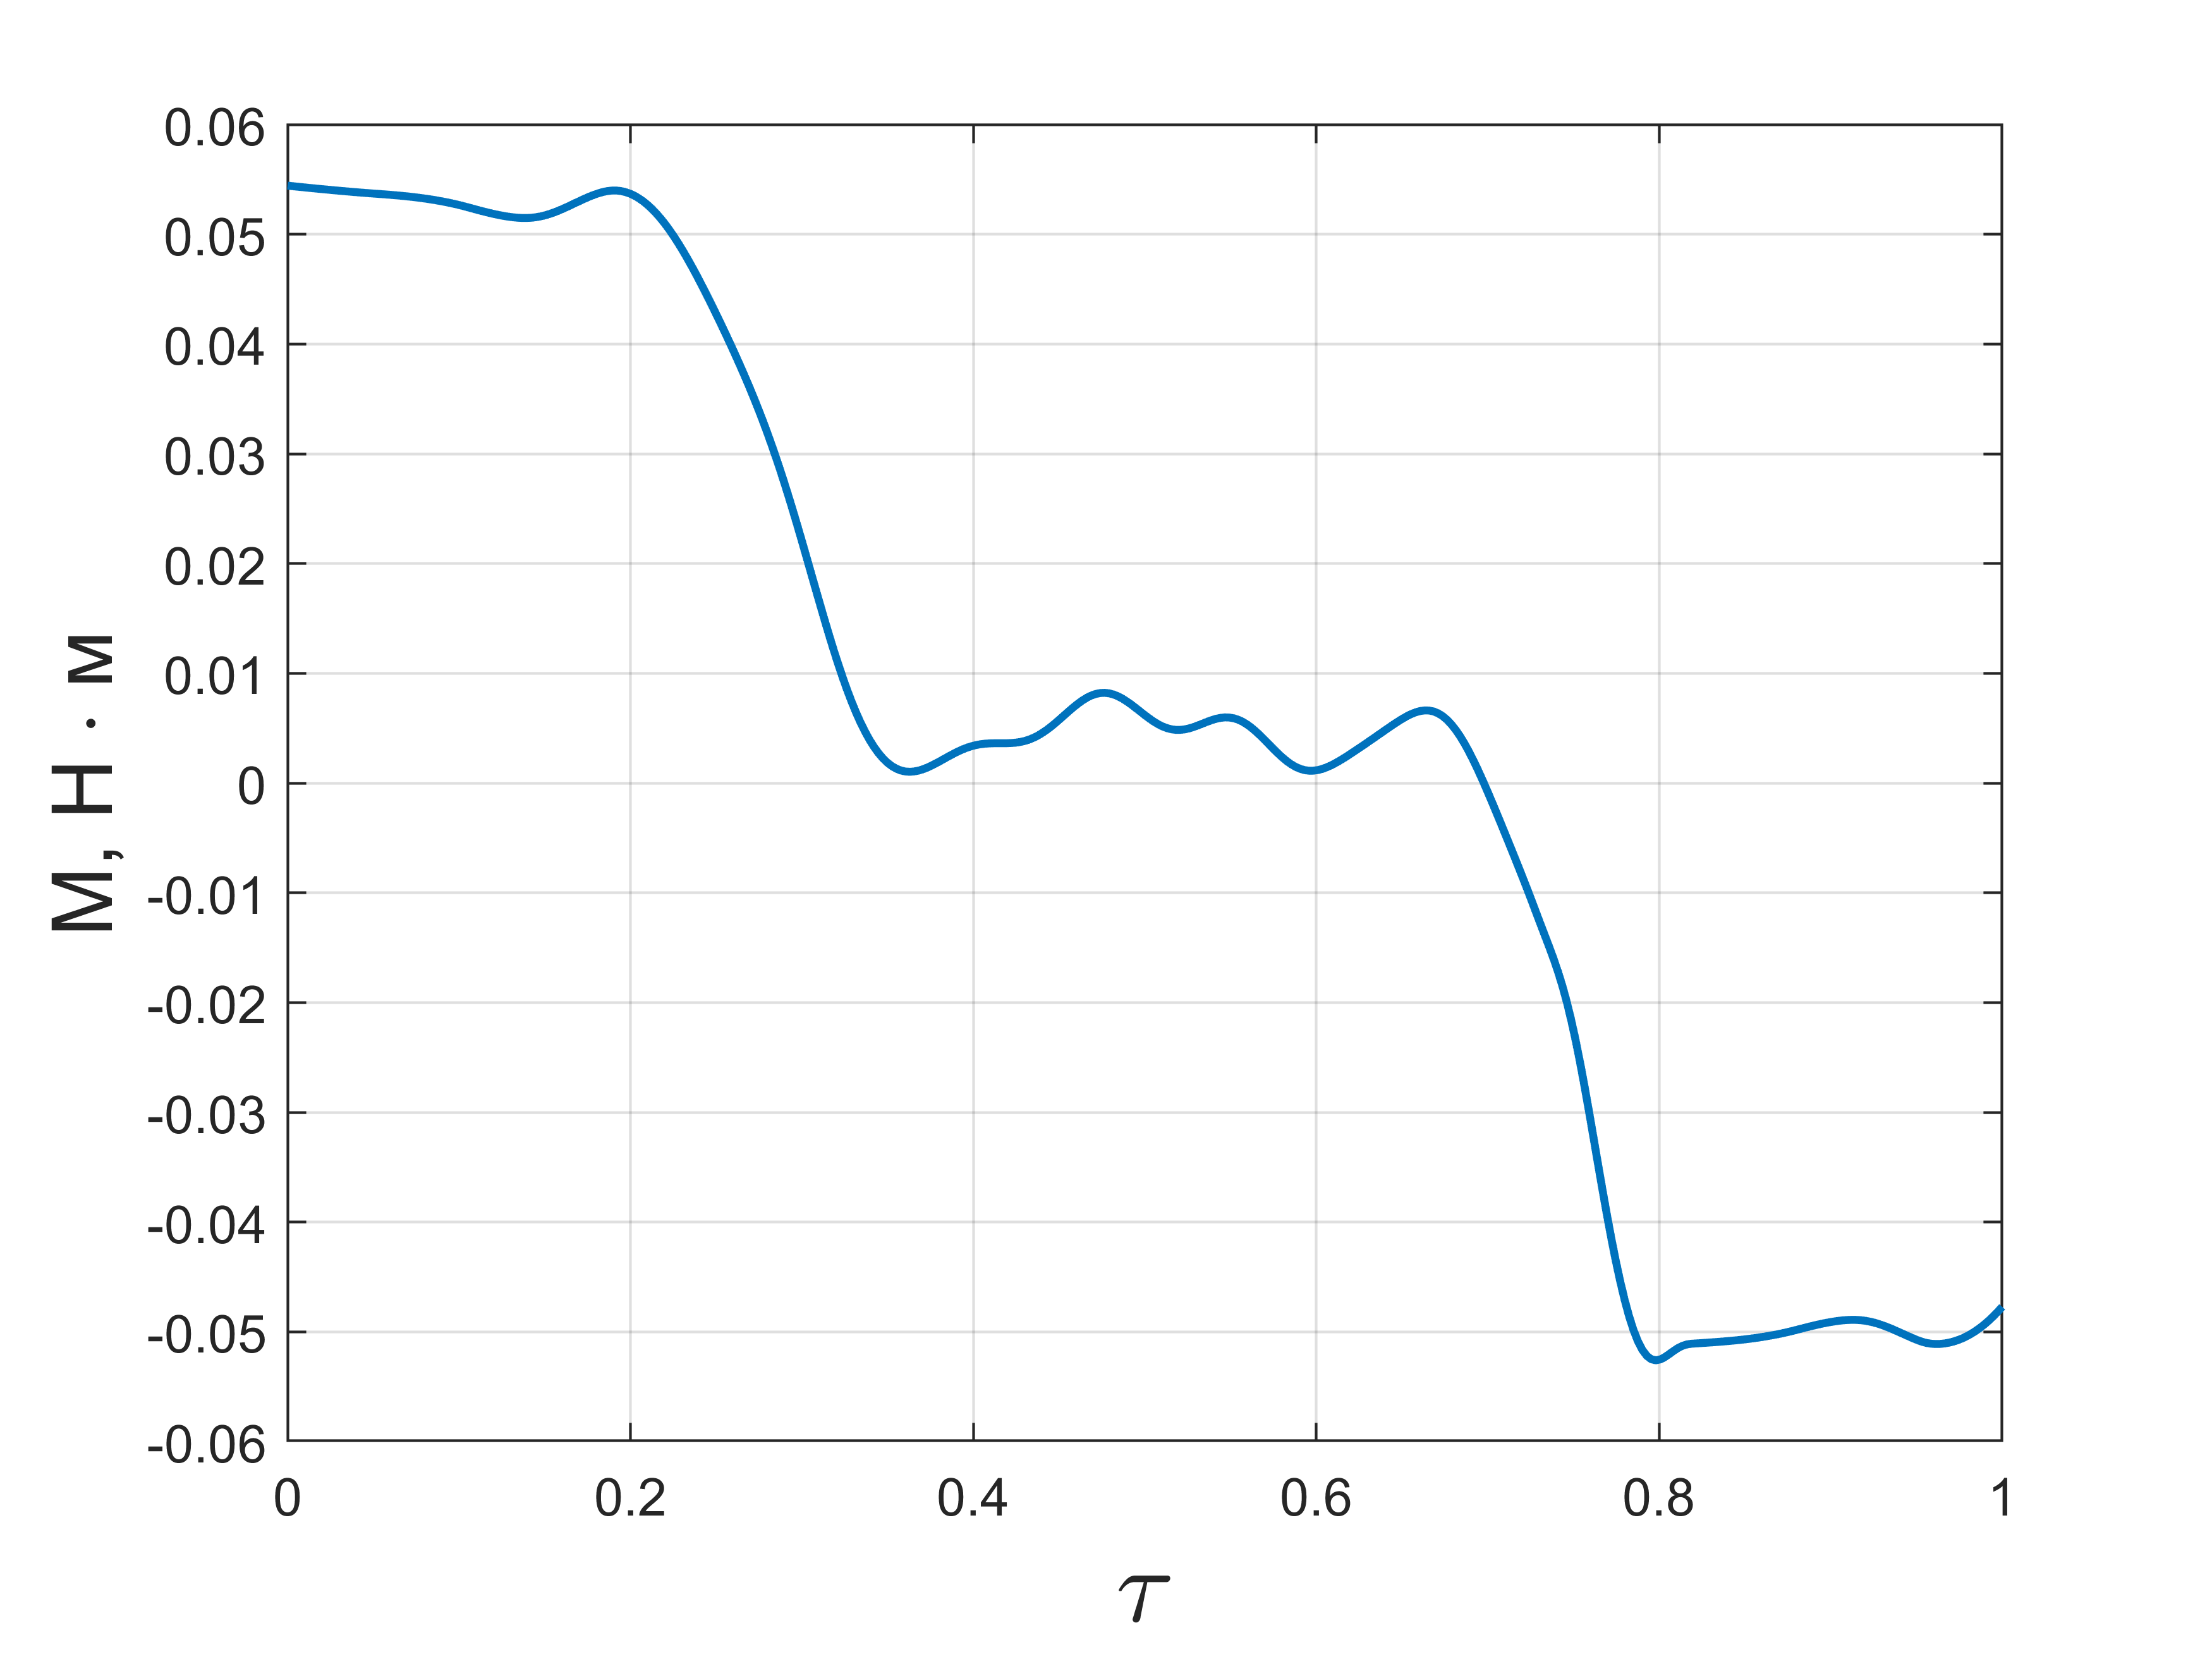
\includegraphics[width=0.8\linewidth]{matlab/img/oz-gyro-mom.png}\\[-2pt] б)
	\end{minipage}
	\caption{Реактивный момент при поворотах вокруг а) $OZ$ б) $OY$}
	\label{fig:omn-mom}
\end{figure}

Для усиления компенсации были подобраны и установлены дополнительные балансировочные кольца на маховики  по осям $OY$ и $OZ$ с моментами инерции, равными $J_{my}=\num{0.0015}\,\si{\kilo\gram\meter\squared}$ и $J_{mz}=\num{0.0011}\,\si{\kilo\gram\meter\squared}$ соответственно. После установки колец проведены повторные стендовые измерения с использованием синусоидального профиля разгона привода.


На рисунке~\cref{fig:sin-profile-omn} представлены результаты измерений после установки балансировочных колец и применения синусоидального профиля.
\begin{figure}[h!]
	% --- Первая строка ---
	\begin{minipage}[b]{0.49\linewidth}\centering
		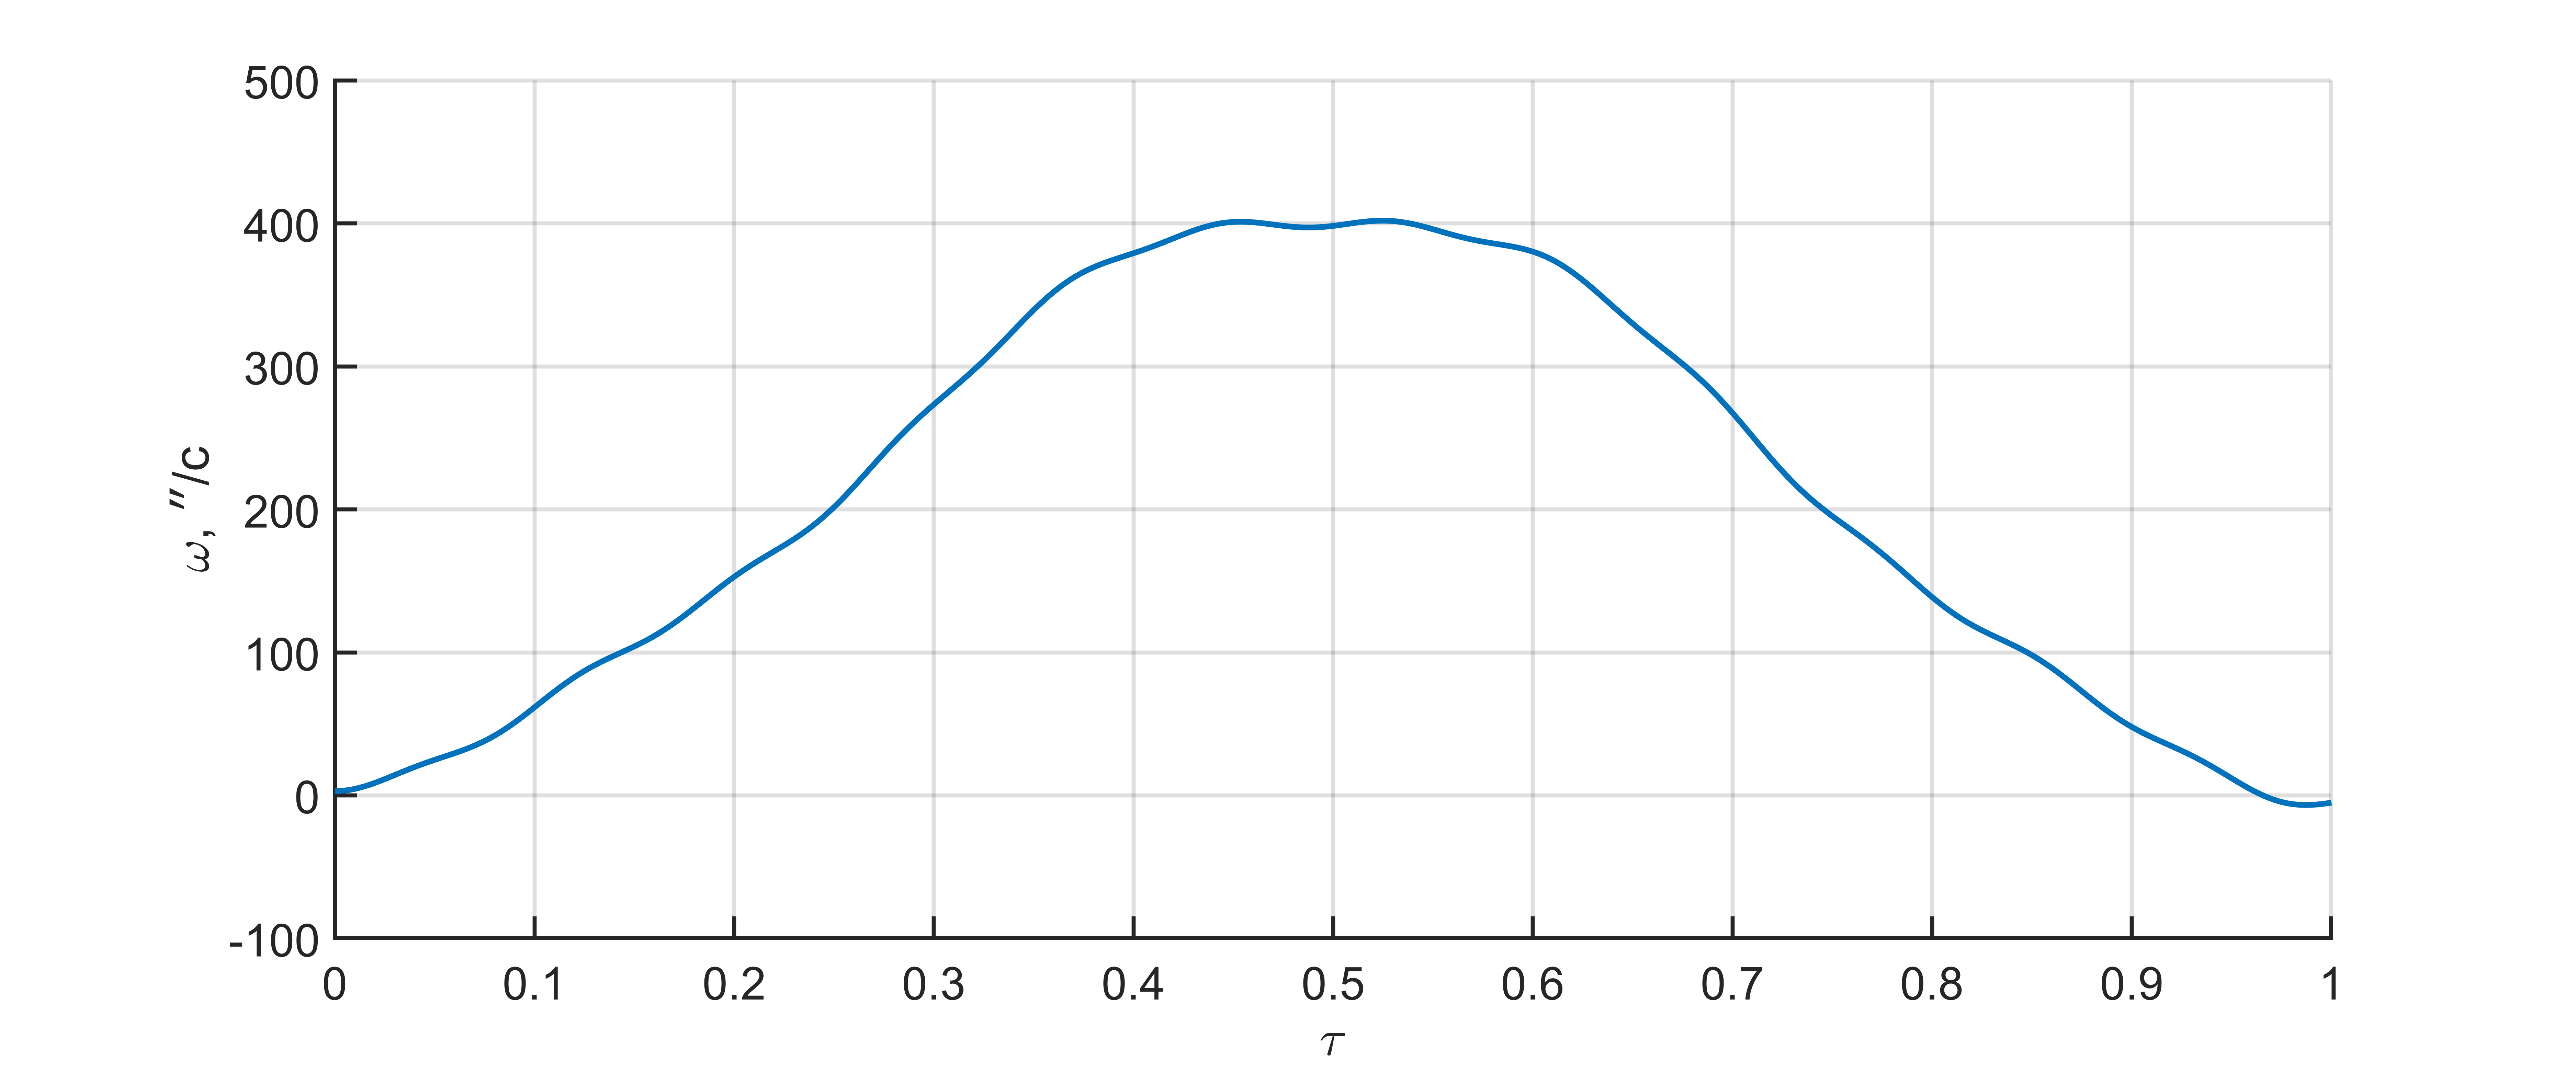
\includegraphics[width=\linewidth]{matlab/img/oz-gyro-sin-vel} \\ а) угловая скорость (ось $OZ$)
	\end{minipage}
	\hfill
	\begin{minipage}[b]{0.49\linewidth}\centering
		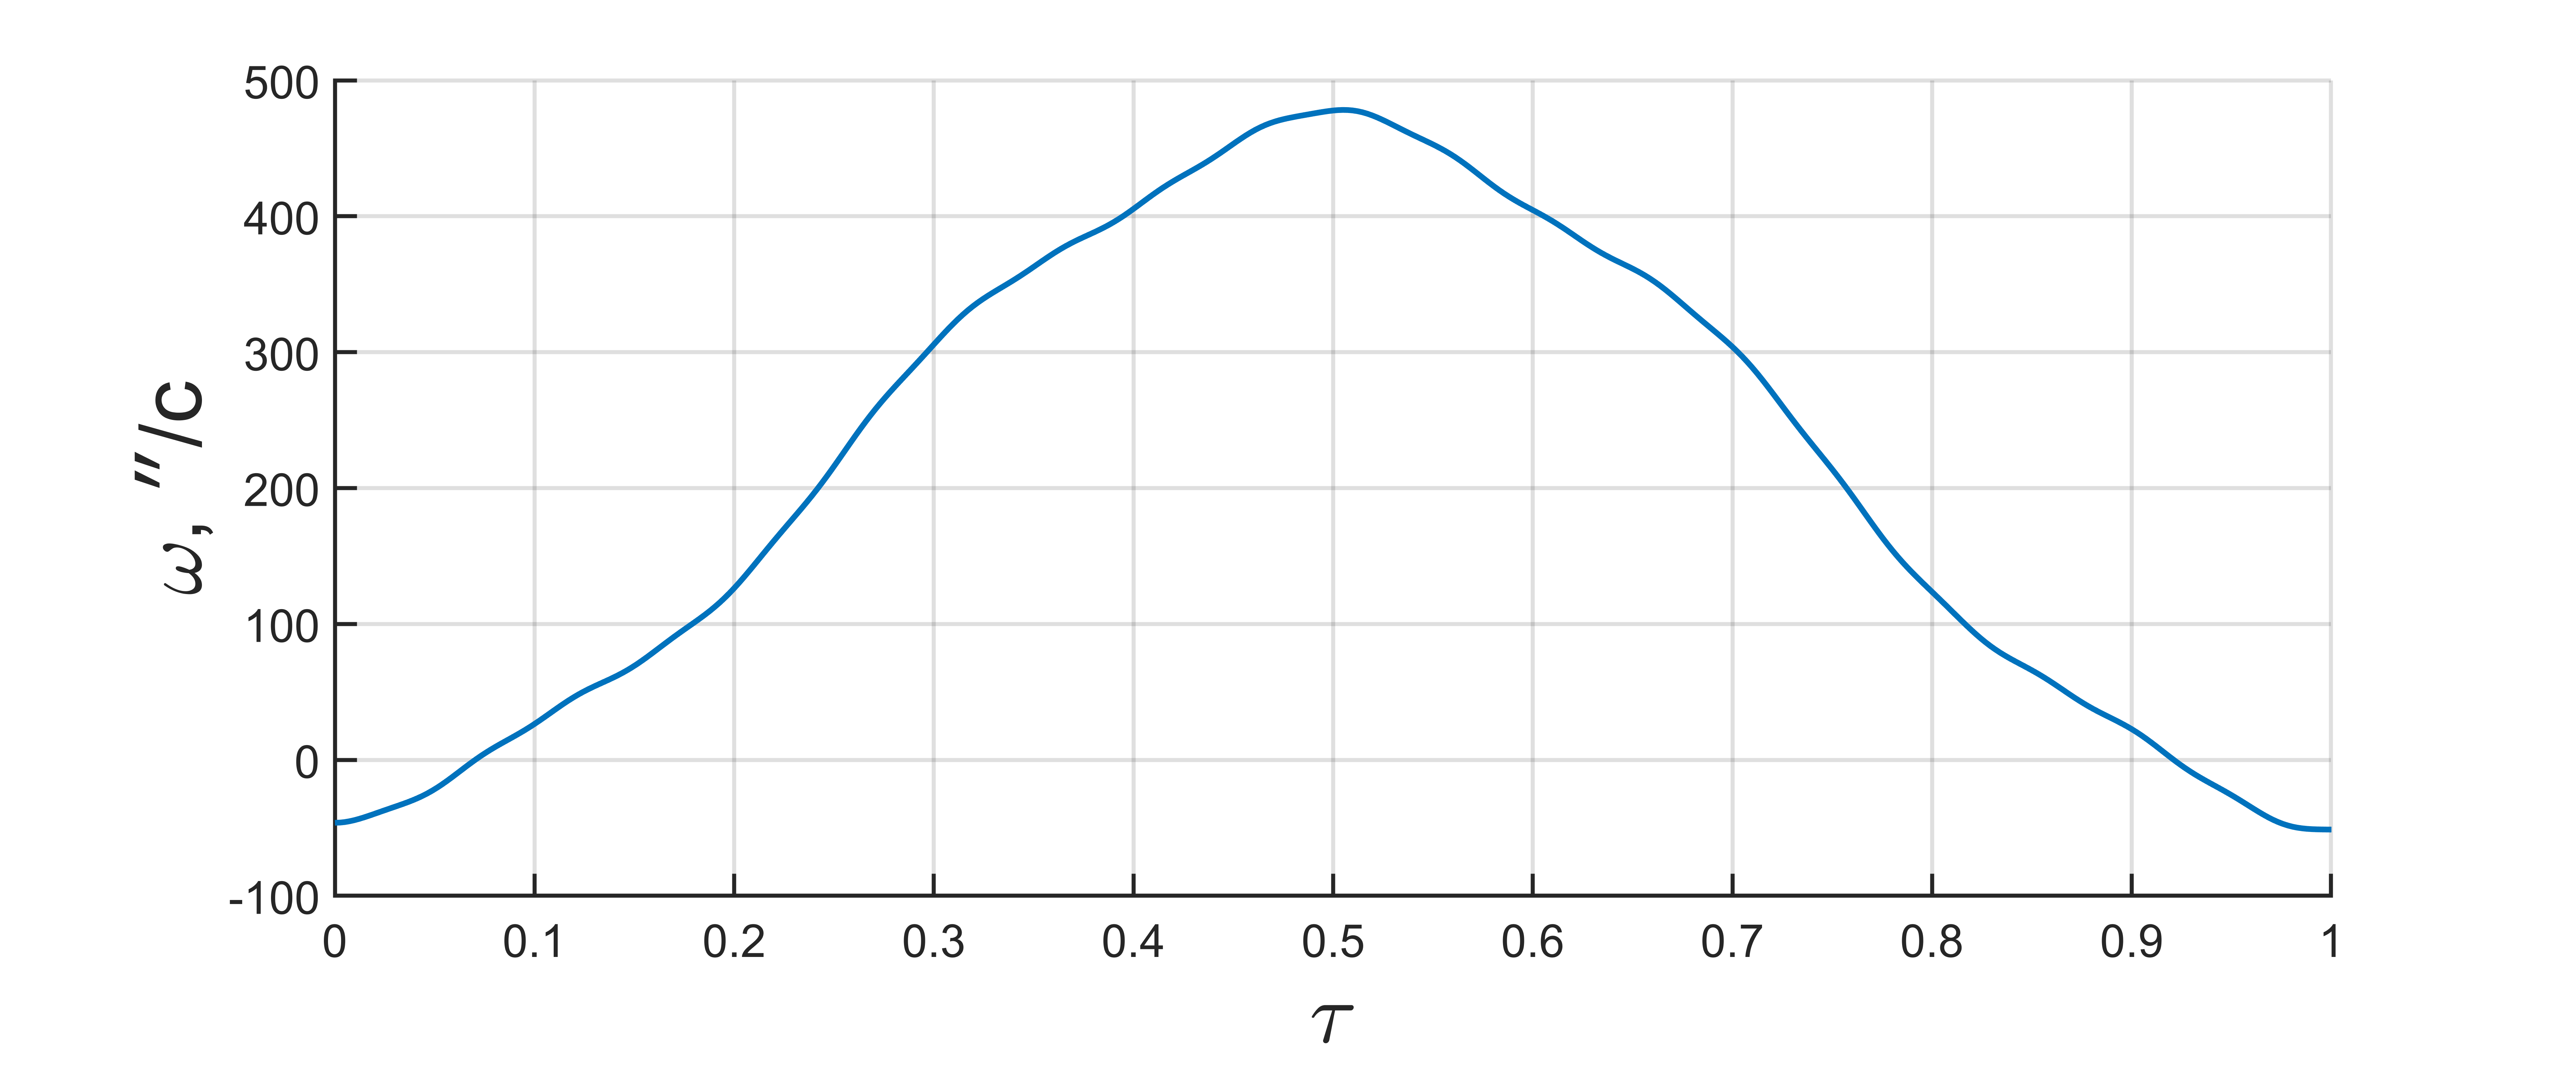
\includegraphics[width=\linewidth]{matlab/img/oy-gyro-sin-vel} \\ б) Угловая скорость (ось $OY$)
	\end{minipage}
	
	\vspace{0.5em} % расстояние между строками
	
	% --- Вторая строка ---
	\begin{minipage}[b]{0.49\linewidth}\centering
		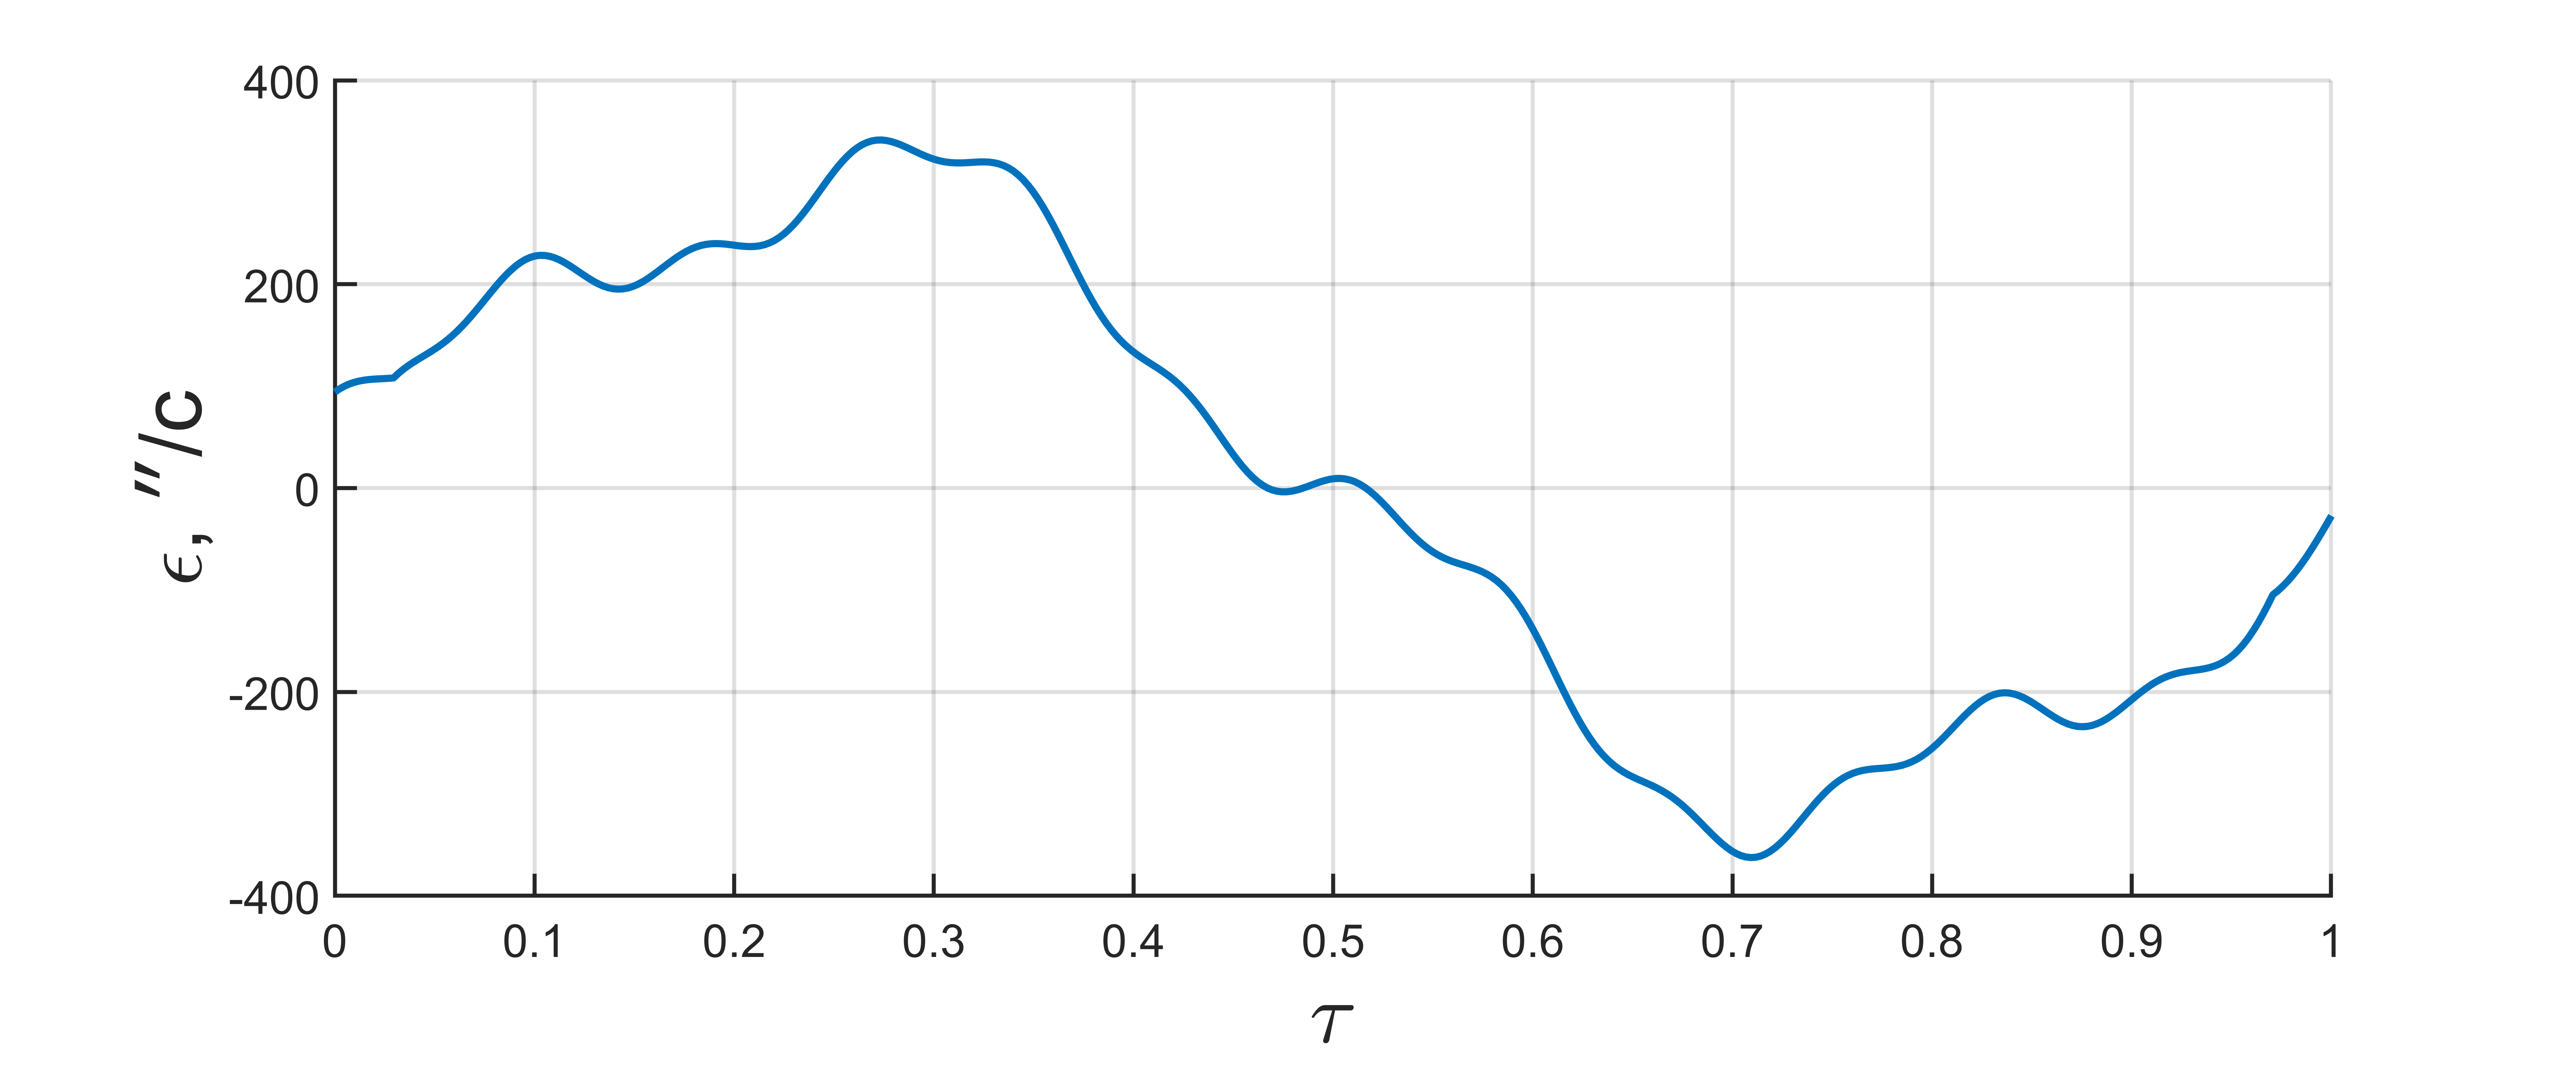
\includegraphics[width=\linewidth]{matlab/img/oz-gyro-sin-acc} \\ в) угловое ускорение (ось $OZ$)
	\end{minipage}
	\hfill
	\begin{minipage}[b]{0.49\linewidth}\centering
		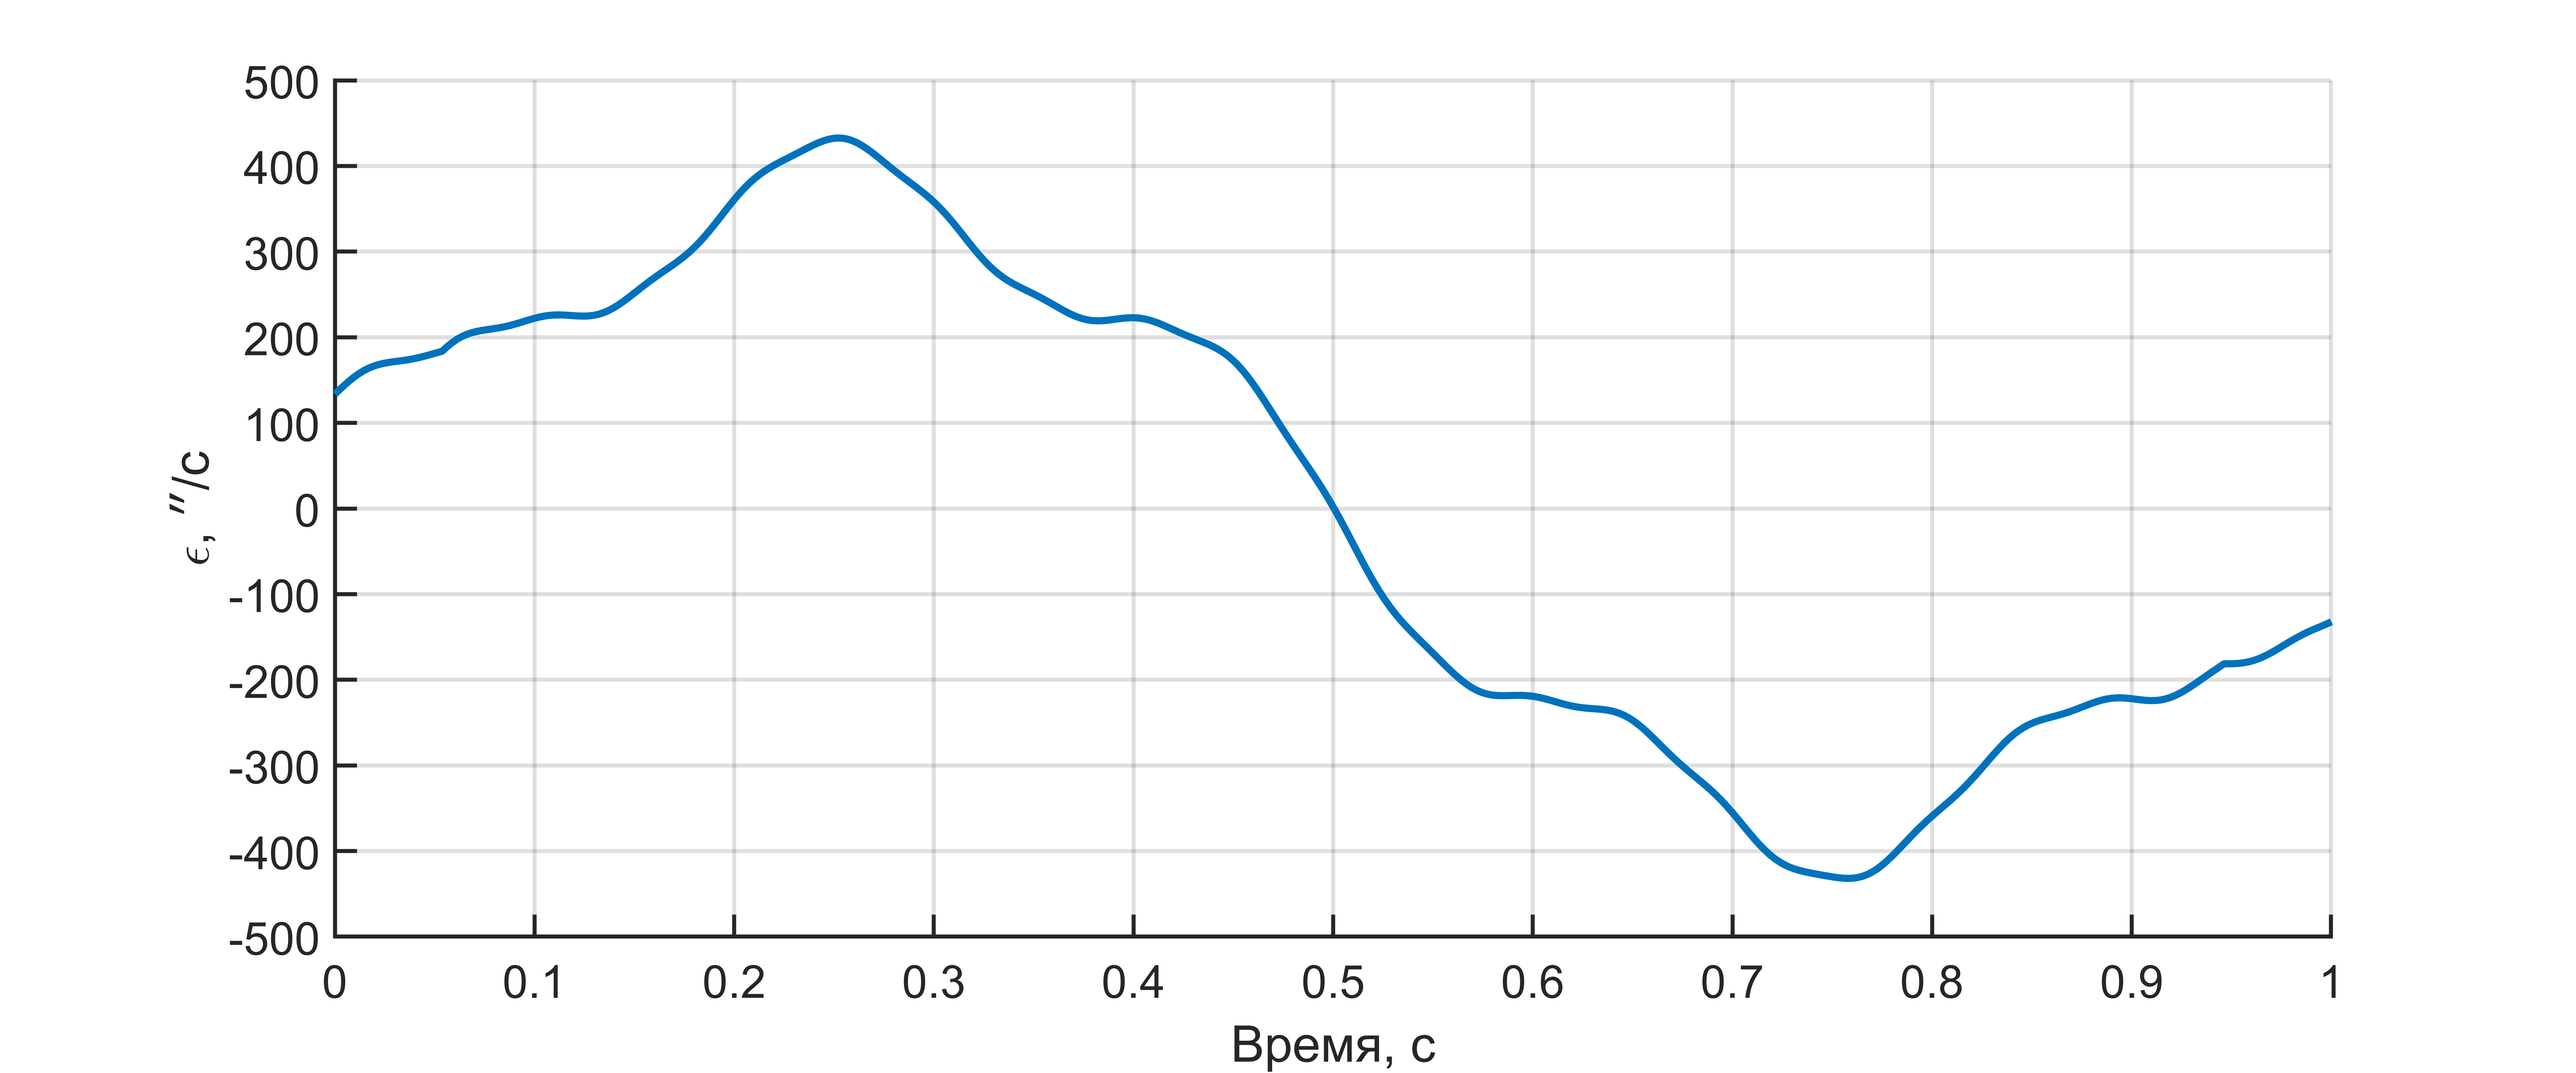
\includegraphics[width=\linewidth]{matlab/img/oy-gyro-sin-acc} \\ г)  угловое ускорение (ось $OY$)
	\end{minipage}
	
	\vspace{0.5em} % расстояние между строками
	
	\begin{minipage}[b]{0.49\linewidth}\centering
		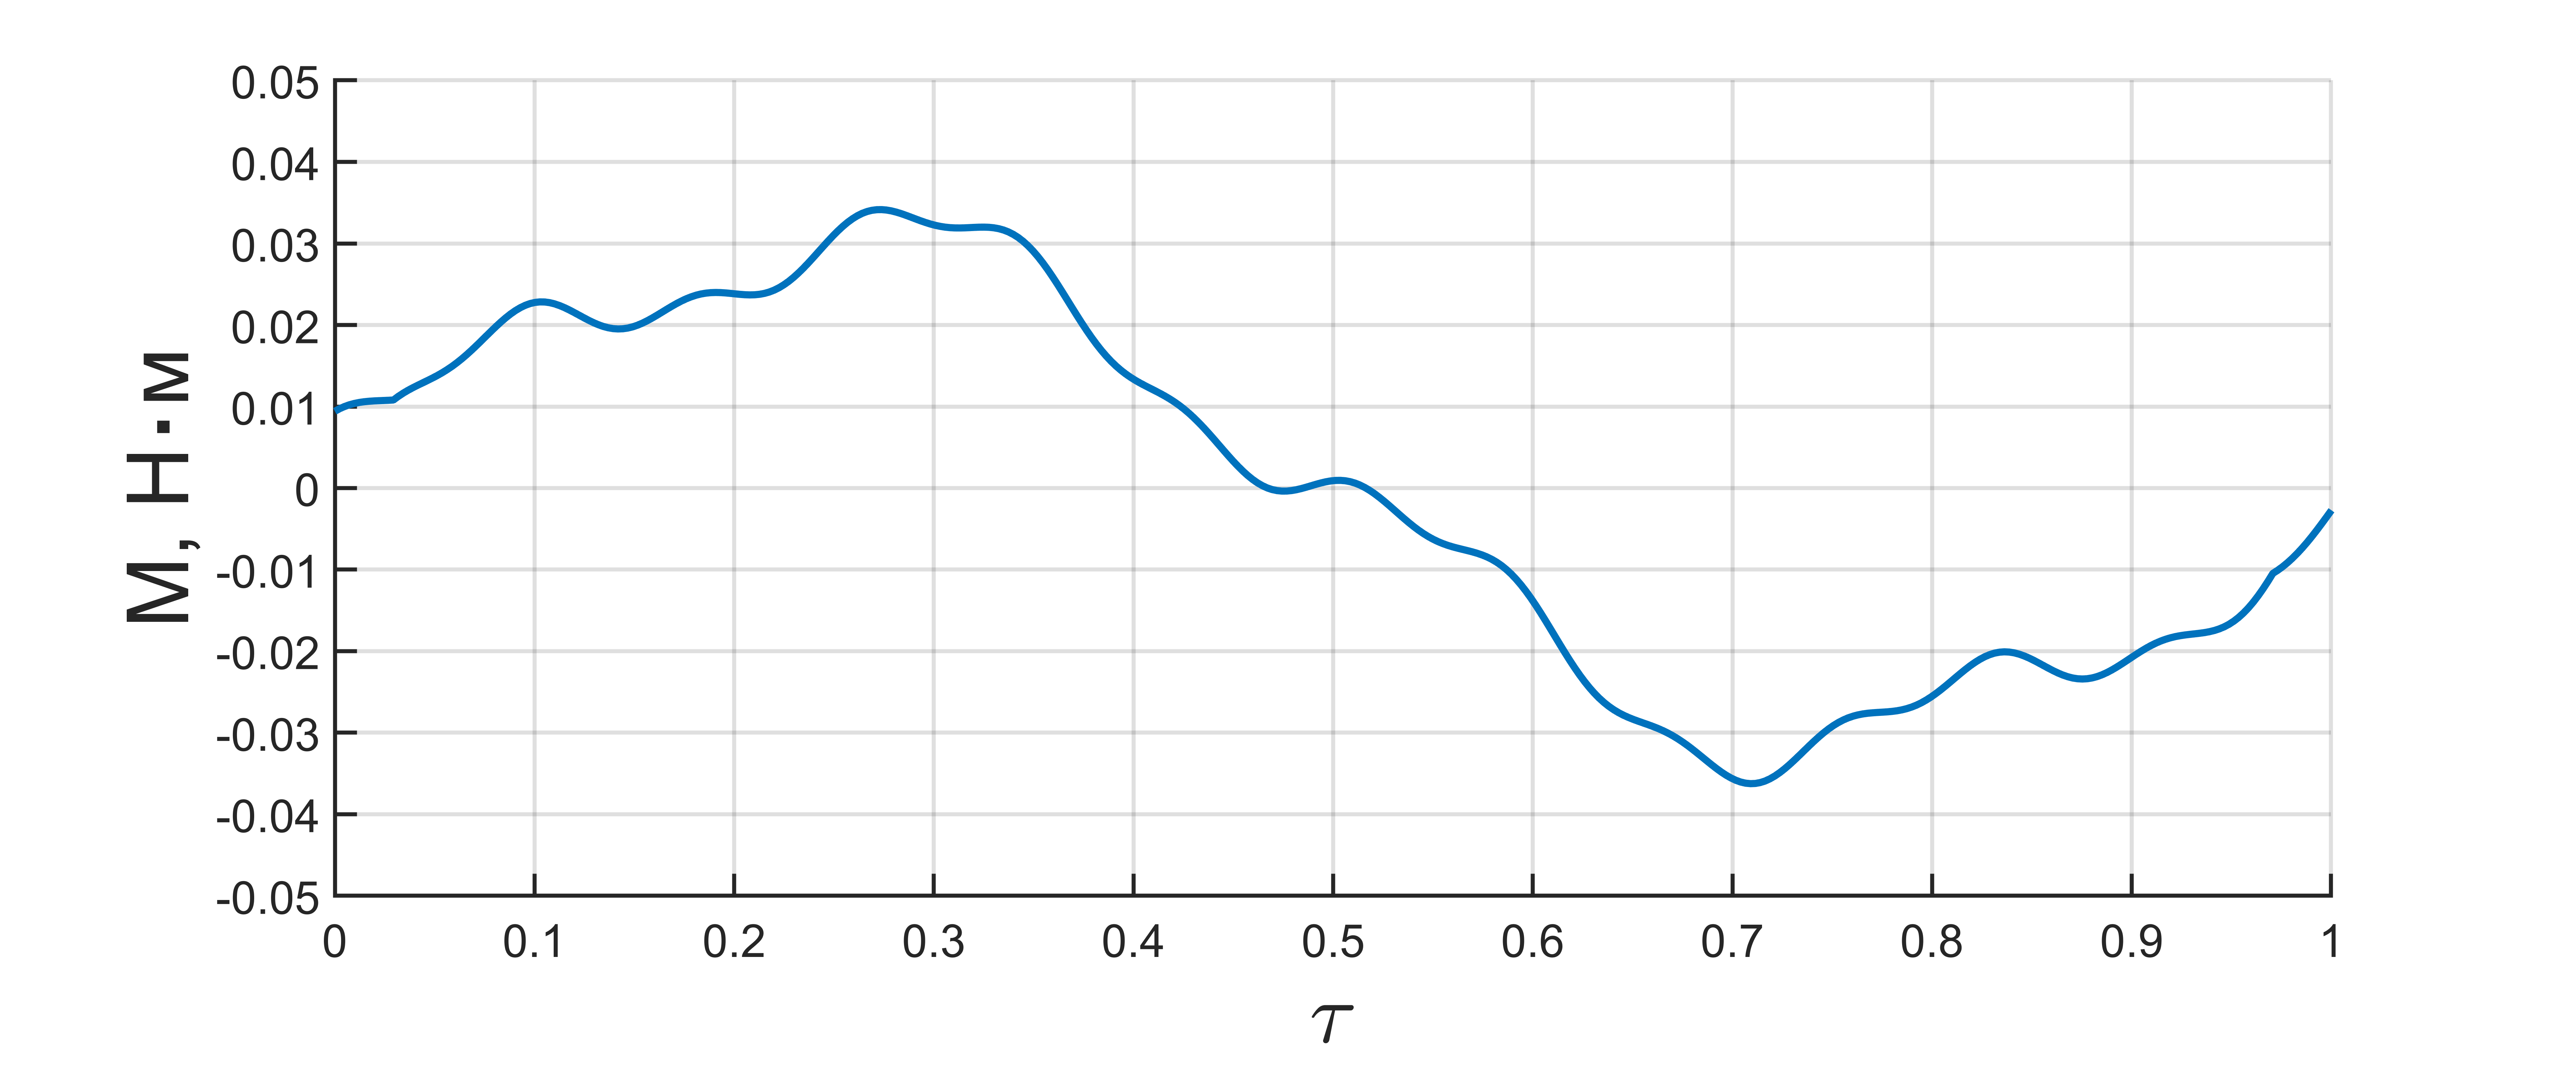
\includegraphics[width=\linewidth]{matlab/img/oz-gyro-sin-mom} \\ д) реактивный момент (ось $OZ$)
	\end{minipage}
	\hfill
	\begin{minipage}[b]{0.49\linewidth}\centering
		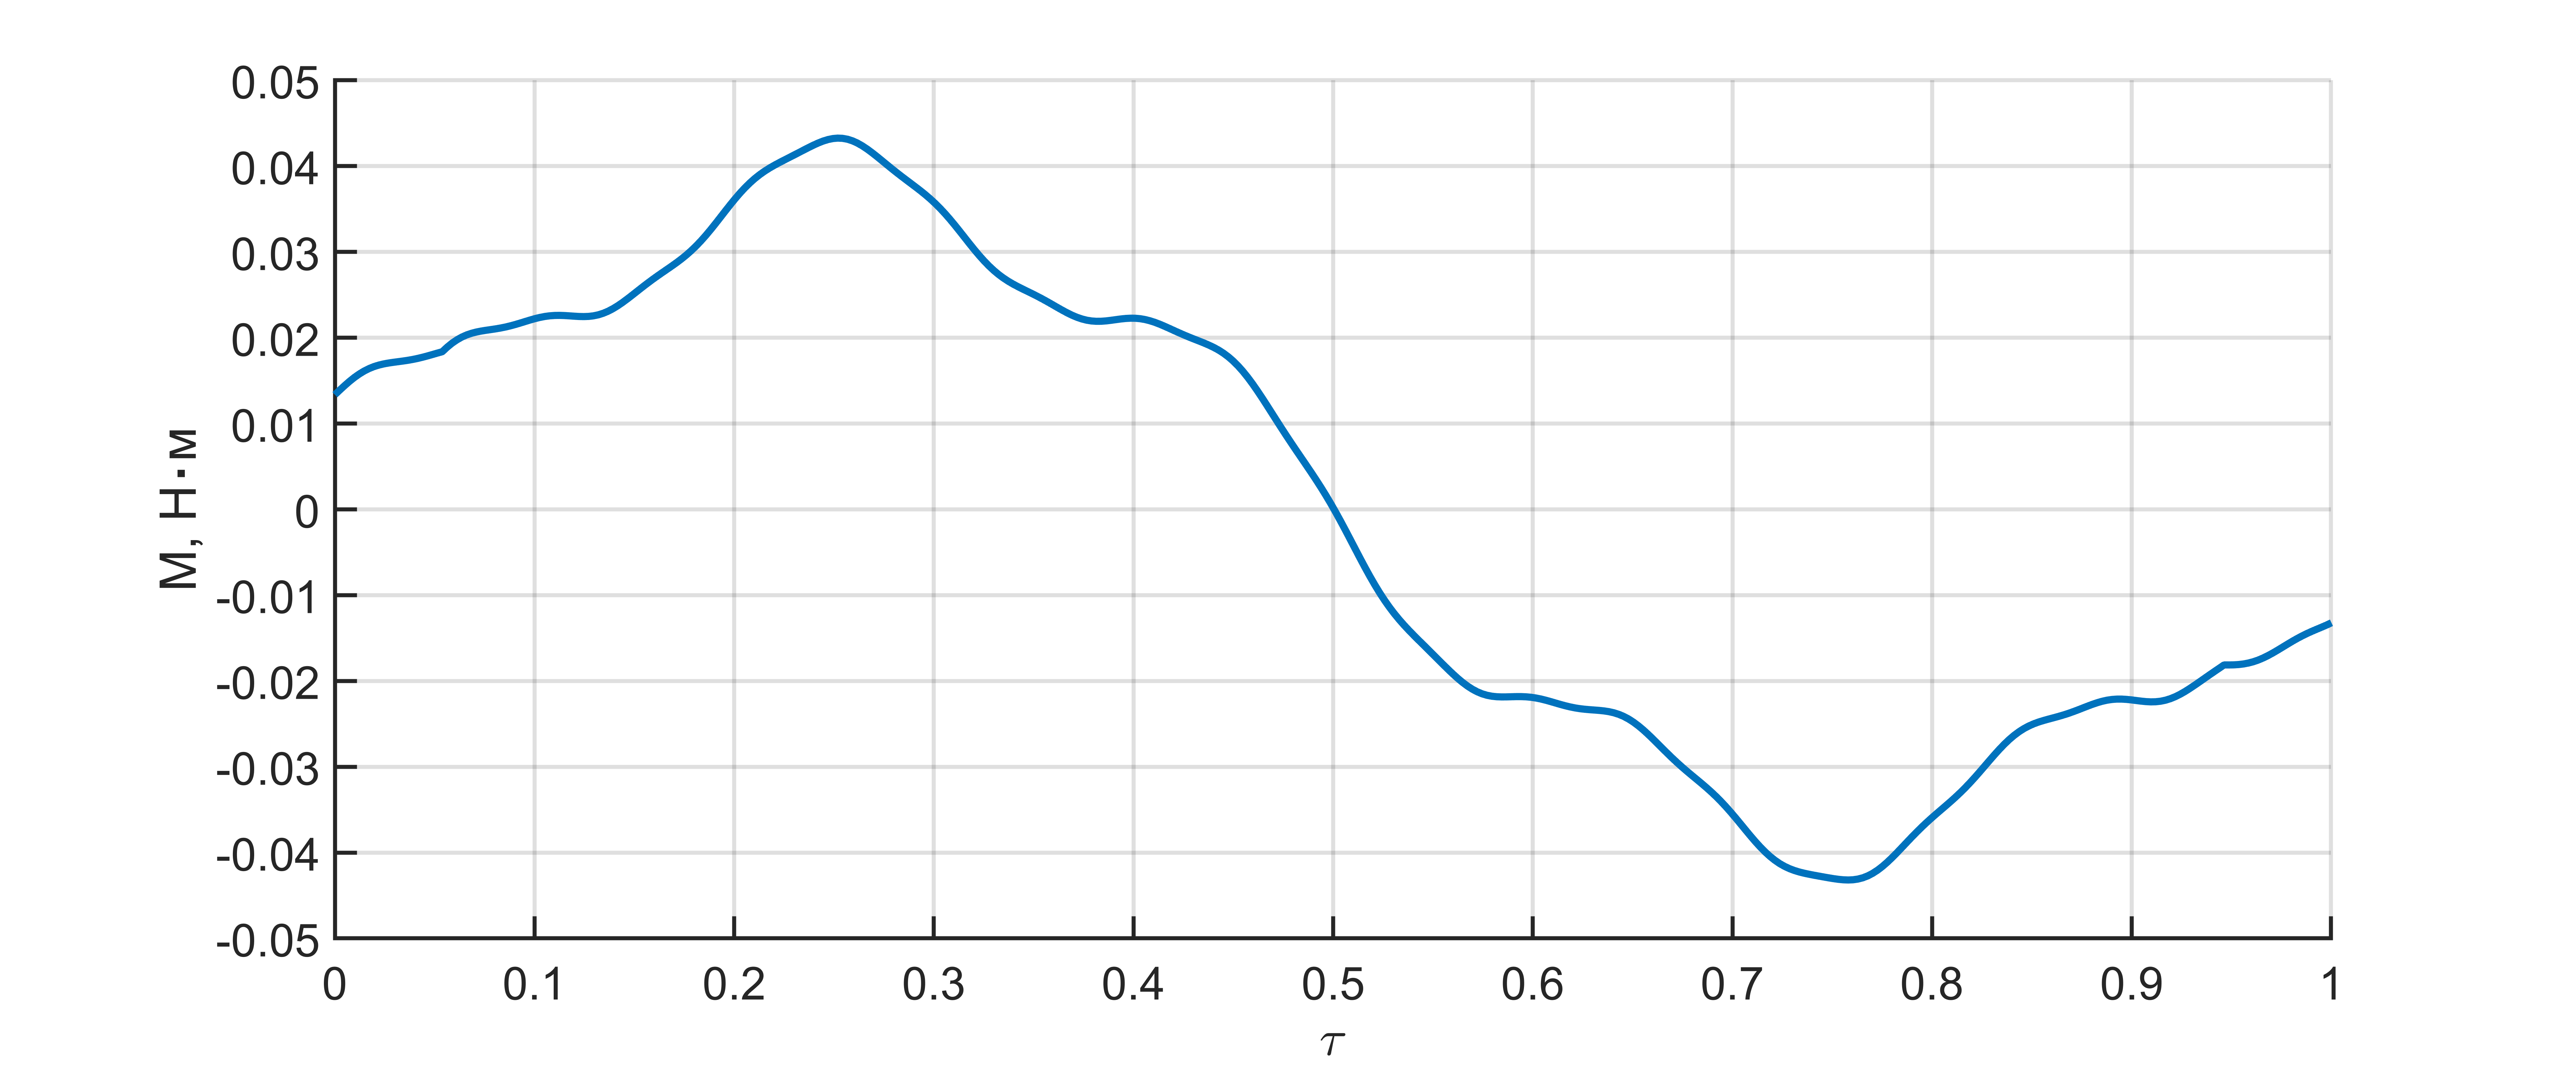
\includegraphics[width=\linewidth]{matlab/img/oy-gyro-sin-mom} \\ е)  реактивный момент (ось $OY$)
	\end{minipage}
	
	\caption{Измерения после установки балансировочных колец}
	\label{fig:sin-profile-omn}
\end{figure}

Сравнение полученных зависимостей с результатами первой серии испытаний показало, что после установки балансировочных колец величина реактивного момента снизилась, а форма кривых стала более симметричной и плавной. Применение синусоидального профиля управления дополнительно уменьшило амплитуду ускорений и сгладило переходные процессы, что привело к снижению возбуждения колебаний подвесной системы. Таким образом, доработанная конструкция МНО в сочетании с оптимизированным законом управления обеспечивает более эффективную компенсацию реактивного момента и повышает точность стабилизации оптической системы.

Доработанный таким образом лётный образец МНО был запущен на орбиту. Для оценки влияния остаточного реактивного момента в условиях полёта
проанализированы данные бортовых гироскопов КА.

 \begin{figure}[h!]
	\begin{minipage}[b][][b]{0.49\linewidth}\centering
		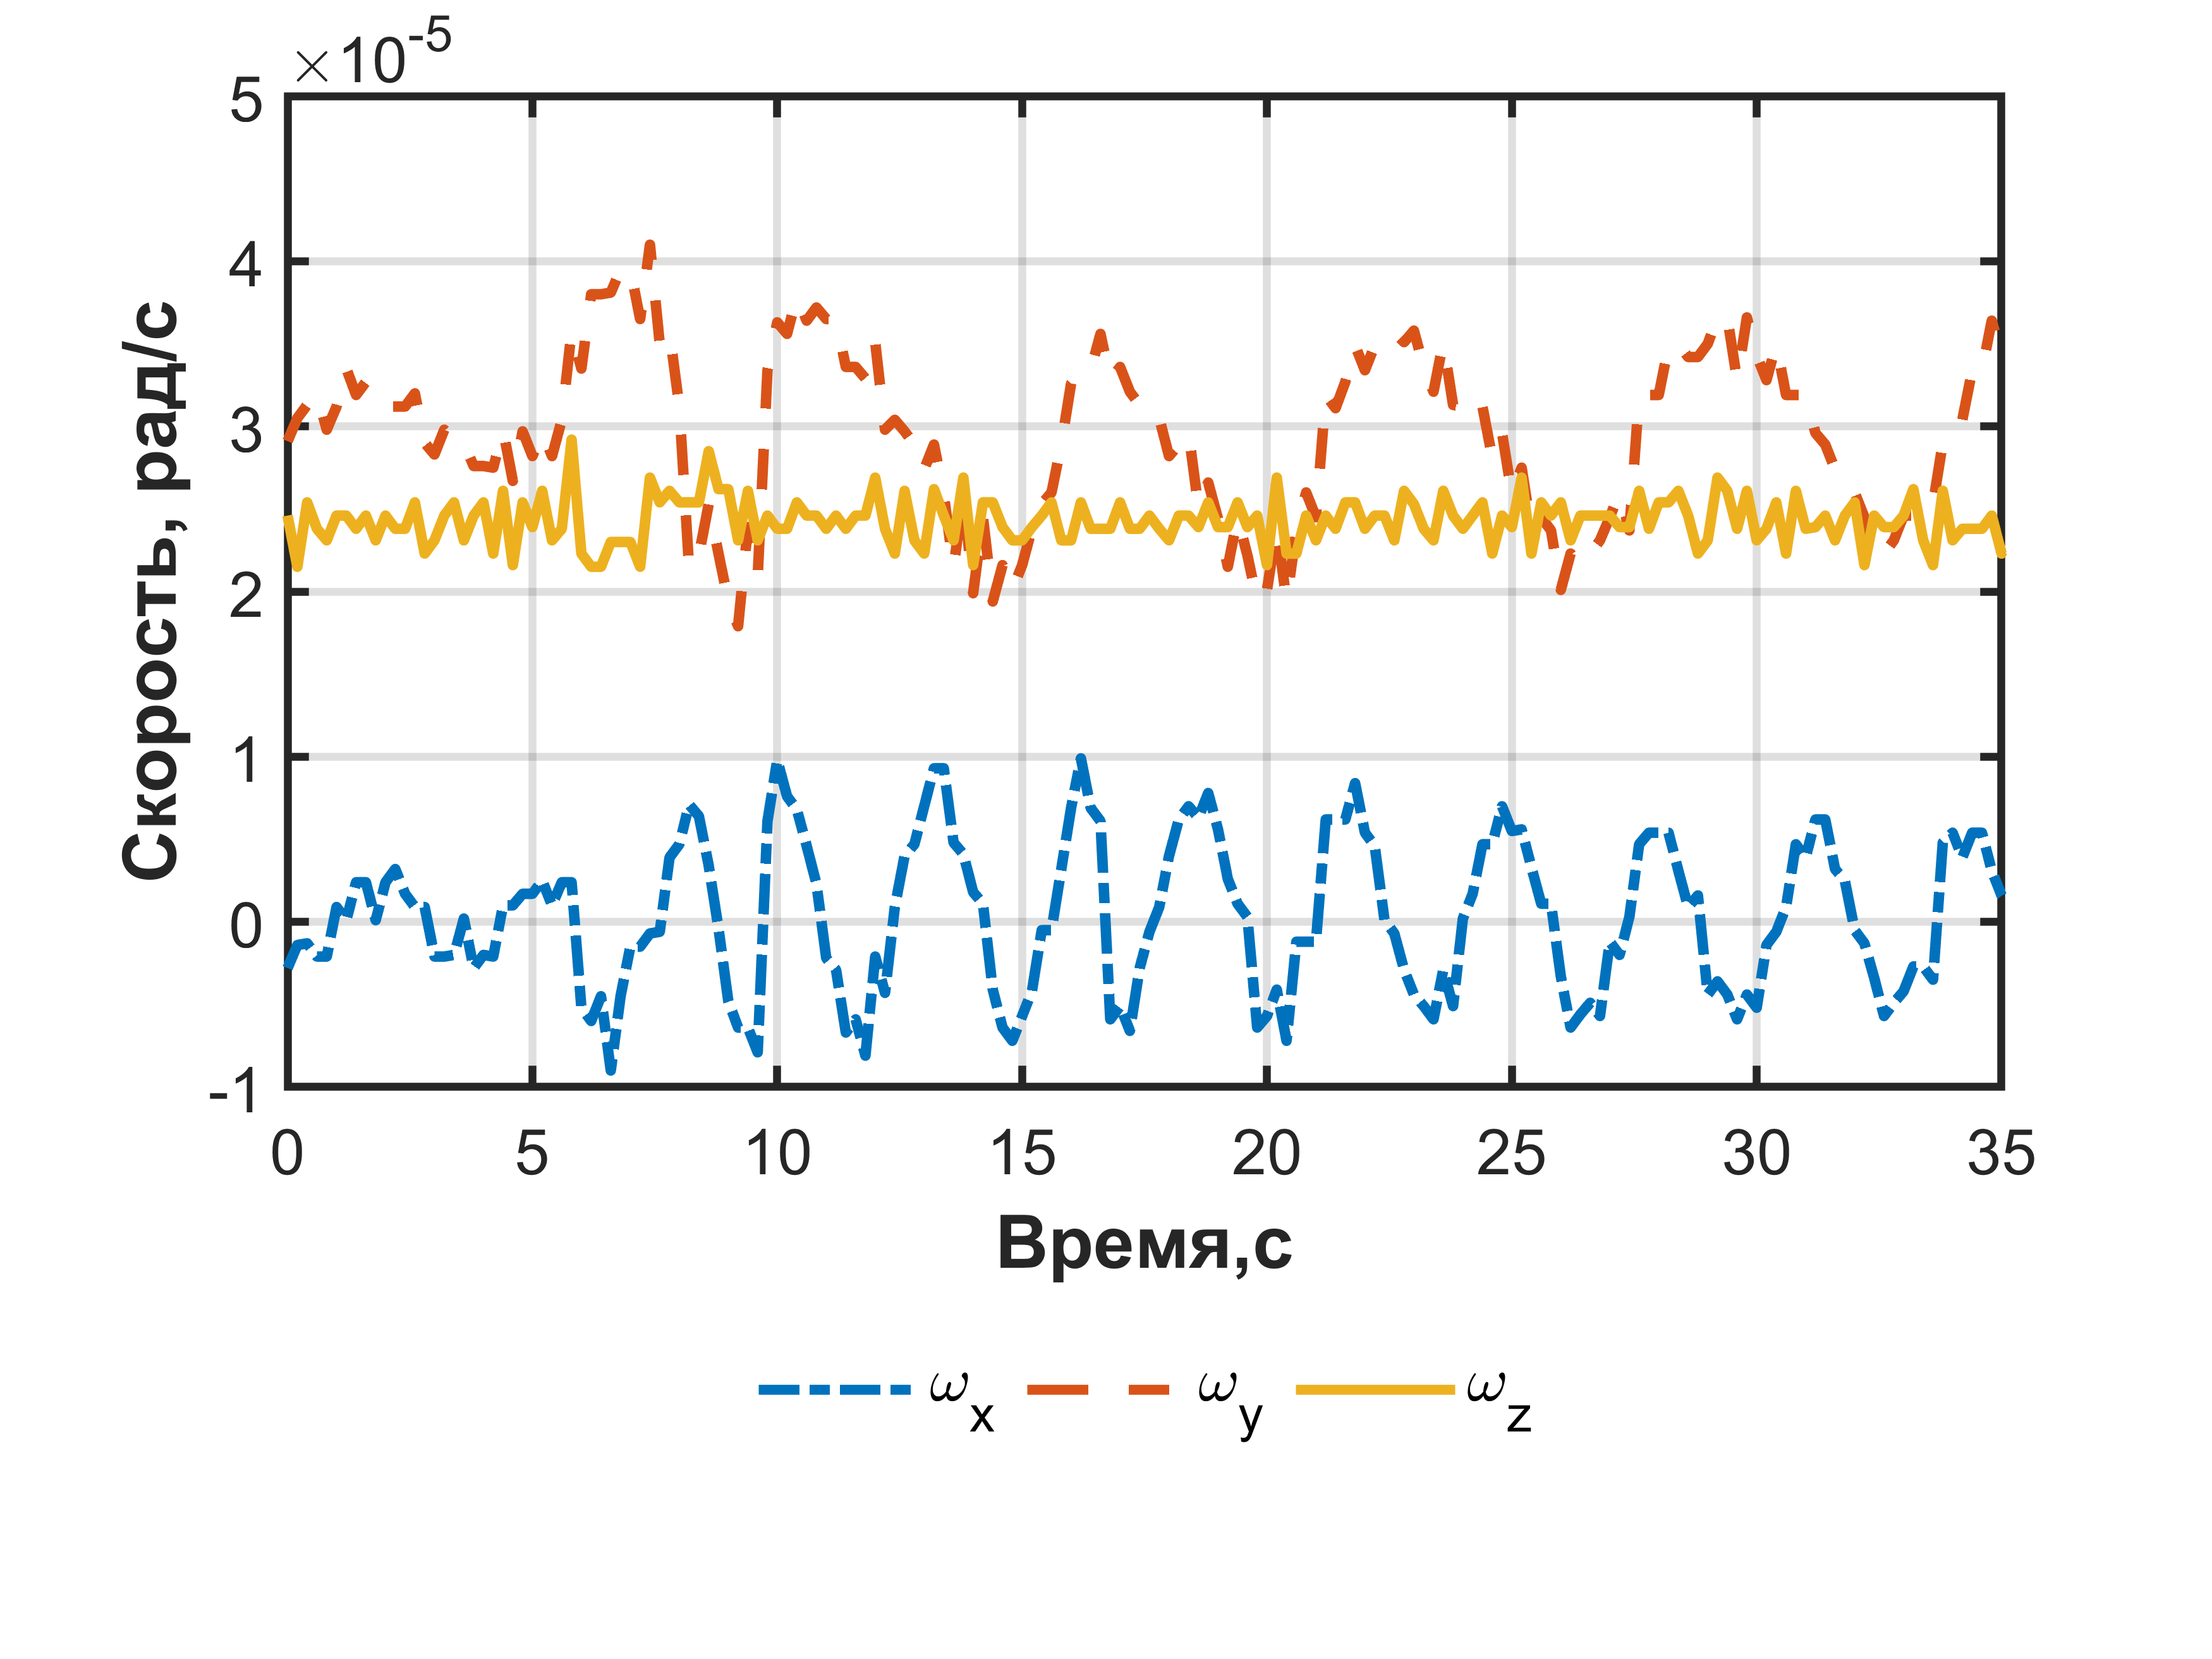
\includegraphics[width=1\linewidth]{matlab/img/sat_gyro_dataY.png} \\ a)
	\end{minipage}
	\hfill
	\begin{minipage}[b][][b]{0.49\linewidth}\centering
		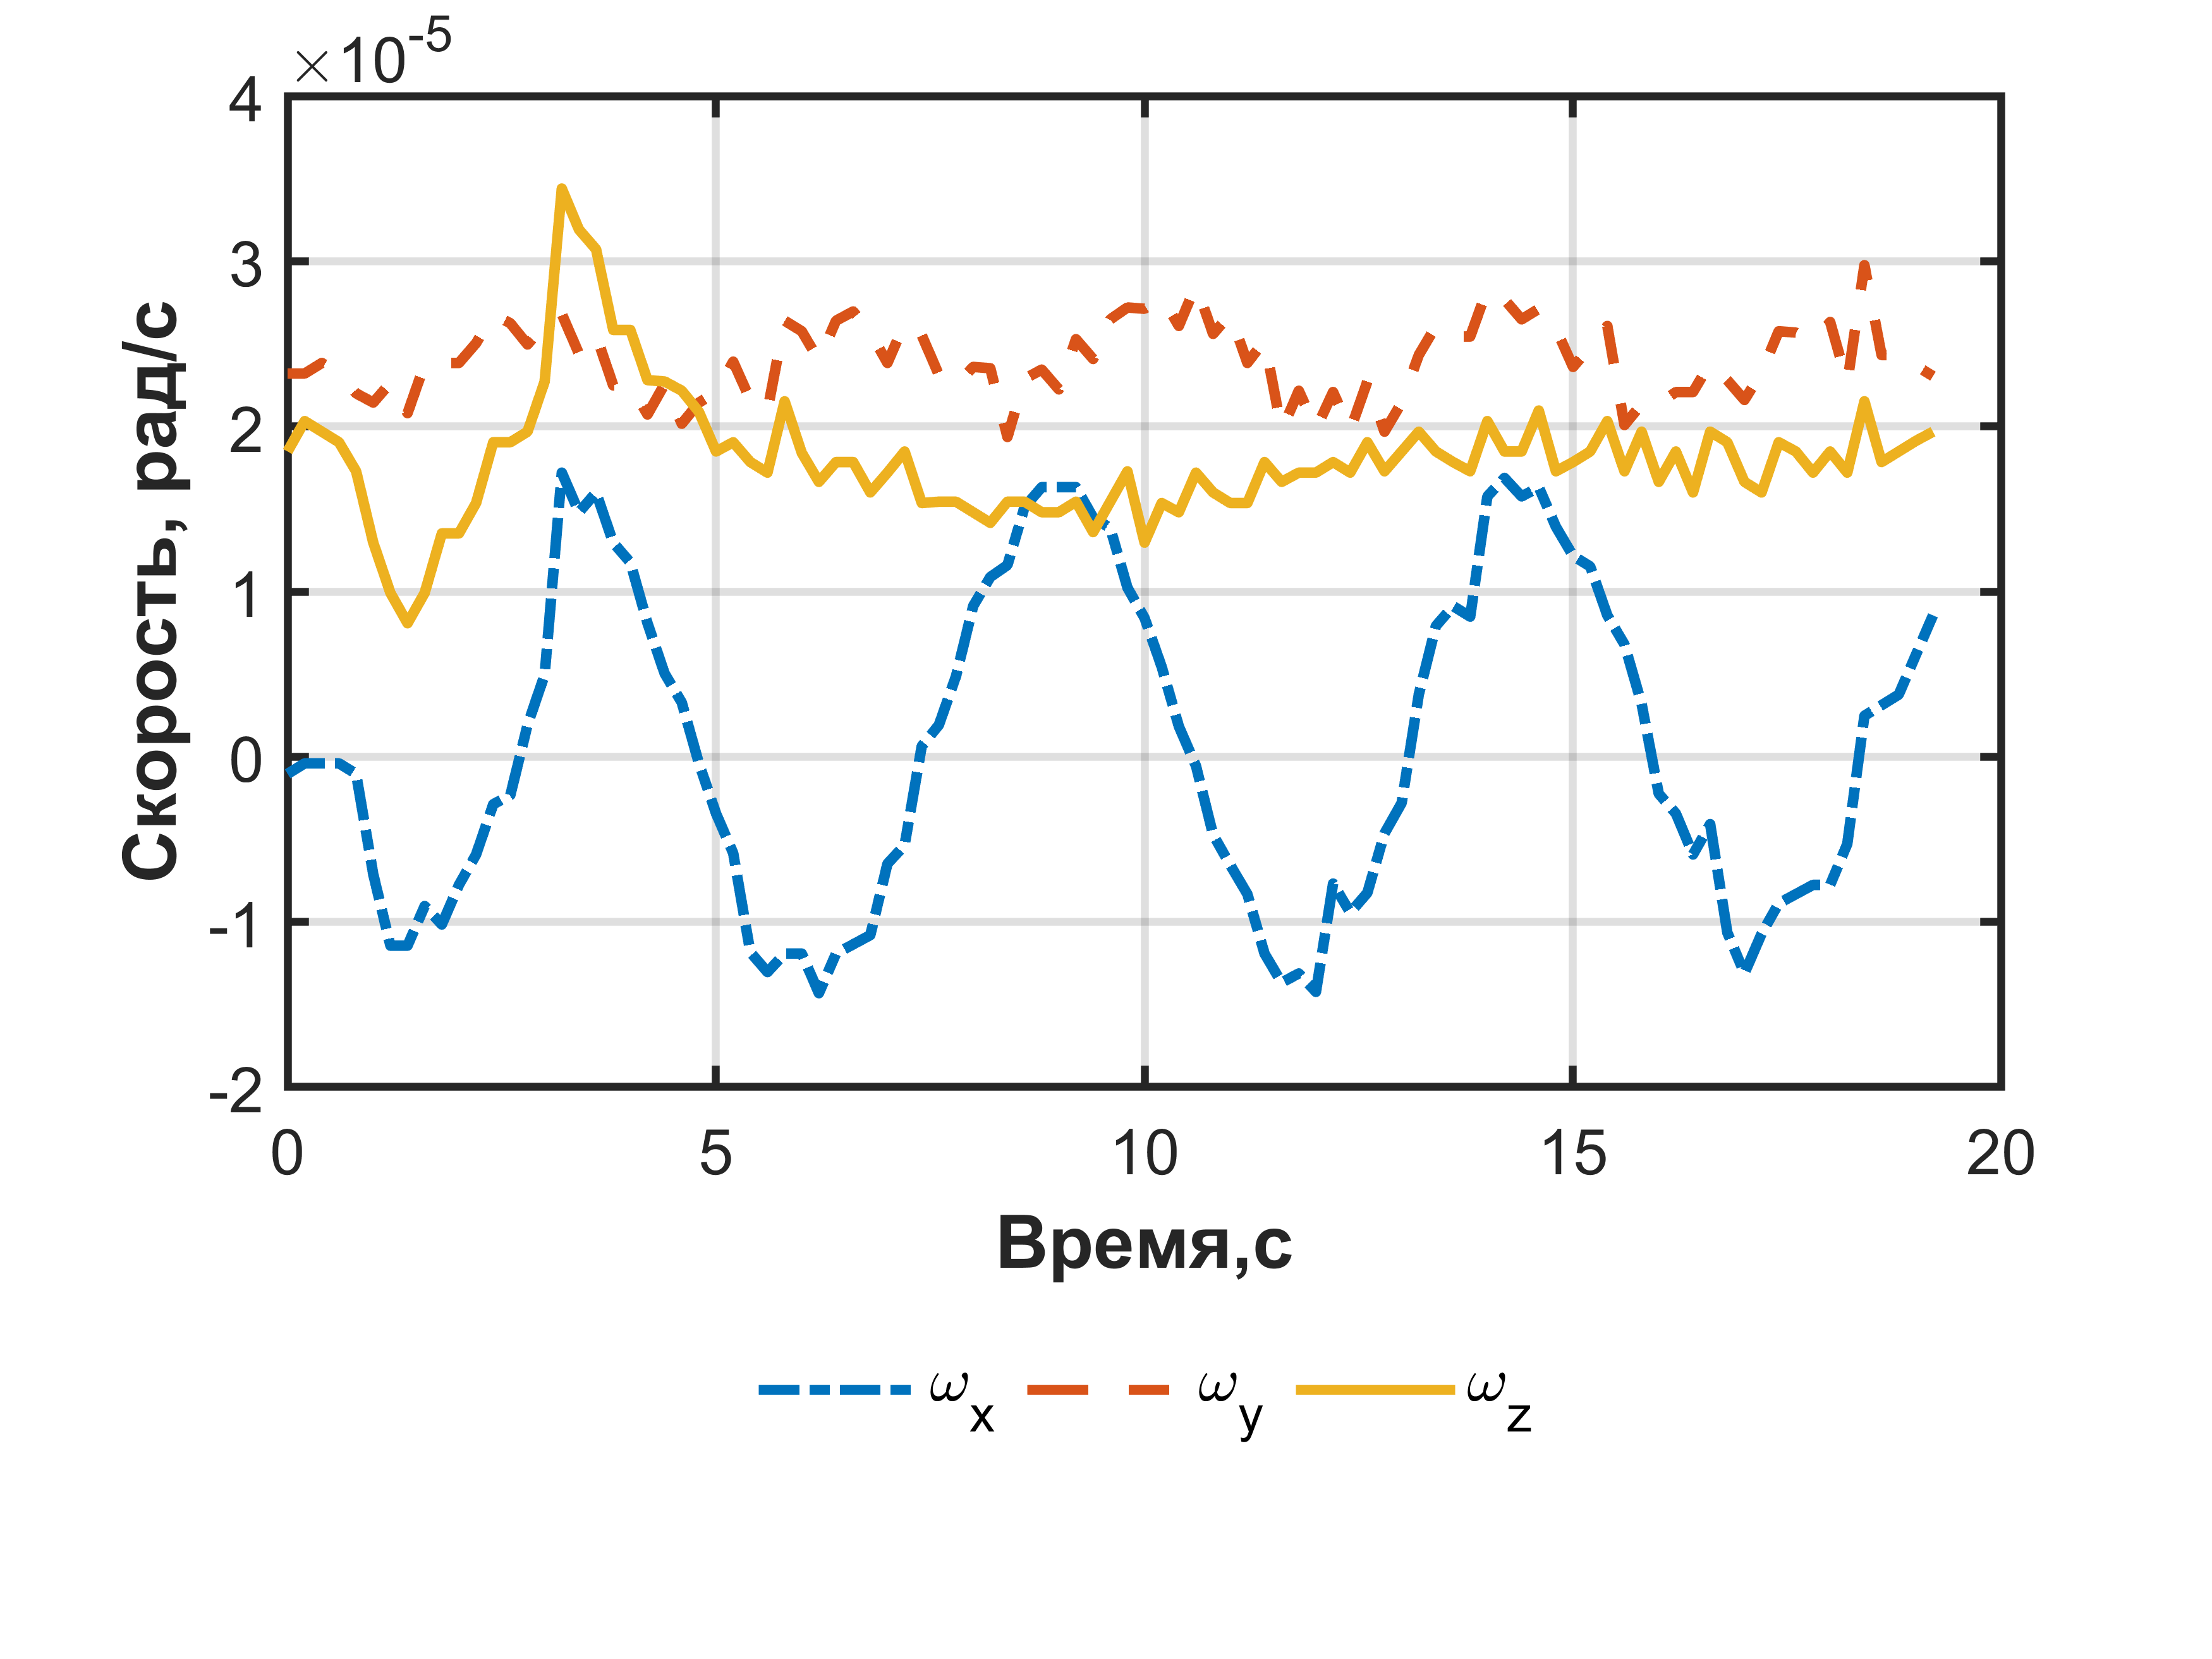
\includegraphics[width=1\linewidth]{matlab/img/sat_gyro_dataZ.png} \\ б)
	\end{minipage}
	\caption{Скорость угловых колебаний спутника при повороте оси визирования по a) оси $OY$, б) оси $OZ$ }
	\label{fig:rotationYZ}
\end{figure}

В моменты максимальных разворотов оси визирования регистрировались угловые скорости
$\omega_y(t), \omega_z(t), \omega_x(t)$ (Рисунок~\cref{fig:rotationYZ}).
Интегрированием получены углы поворота:
\begin{equation}
	\theta_y(t)=\int \omega_y\,dt,\quad
	\theta_z(t)=\int \omega_z\,dt,\quad
	\theta_x(t)=\int \omega_x\,dt.
\end{equation}

Смещение изображения в фокальной плоскости определяется как
\begin{equation}
	\label{eq:bias}
	\mathbf{r}(t) = 
	\begin{bmatrix}
		y(t) \\
		z(t) \\
	\end{bmatrix}
	= f \cdot
	\begin{bmatrix}
		\theta_{y}(t) \\
		\theta_{z}(t)
	\end{bmatrix}
\end{equation}

где $f=\SI{900}{\milli\meter}$ — фокусное расстояние.
За экспозицию $T_{\mathrm{exp}}$ линейное смещение составляет:
 \begin{equation}
	\label{eq:biasL}
	L=\sqrt{(\Delta x)^2+(\Delta y)^2}
\end{equation}
а угловое смещение — $\alpha=R\theta_x$, где $R=\SI{30}{\milli\meter}$ — радиус кадра.
Их совместное действие даёт результирующий сдвиг $L_{\mathrm{tot}}$.

 \begin{equation}
	\label{eq:L_total}
	L_{tot} = \sqrt{L^2 + (R\cdot \theta_x)^2 + 2Lr\theta_x\cos{\psi}}
\end{equation}

Расчёты показали смещения
$L_{OY}=\SI{2.13}{\micro\meter}$ и
$L_{OZ}=\SI{3.09}{\micro\meter}$,
что составляет $0.07$ и $0.10$ пикселя.

Деградация контрастно-частотной характеристики оценивается по следующей формуле:
\begin{equation}
	\text{КЧХ}(\nu)=\frac{\sin(\pi\nu L_{\mathrm{tot}})}{\pi\nu L_{\mathrm{tot}}},\qquad
	\nu_N=\frac{1}{2p},
\end{equation}
где $p=\SI{30}{\micro\meter}$ — размер пикселя.

 На частоте Найквиста получены
\[
MTF(\nu_N)_{OY}\approx 0.998,\qquad
MTF(\nu_N)_{OZ}\approx 0.996.
\]

Таким образом, остаточный реактивный момент не оказывает критического
влияния на формирование изображения, что подтверждает эффективность
мер по компенсации. Система компенсации реактивного момента,
параметры которой были оптимизированы с использованием разработанного
измерительного стенда, сводит величину возмущающих воздействий к
уровню, не влияющему на качество изображения.


Разработанный стенд может использоваться не только для исследования модулей с дискретными поворотами, но и для настройки оптических систем с периодическими колебательными движениями зеркал. В качестве примера рассмотрен сканер, в котором компенсация реактивного момента осуществляется отдельным маховиком с собственным приводом. Для таких систем предъявляются повышенные требования: остаточный момент должен быть менее $\SI{0,005}{\newton\meter}$, что требует высокой точности согласования работы обоих приводов.

Испытания на стенде включали подбор момента инерции маховика и настройку фазового совпадения его движения с движением зеркала. Результаты (рис.~\ref{fig:scan-mom}) показали, что после настройки уровень остаточного реактивного момента значительно снизился и соответствовал требуемым нормам.

\begin{figure}[h!]
	\begin{minipage}[b]{0.49\linewidth}\centering
		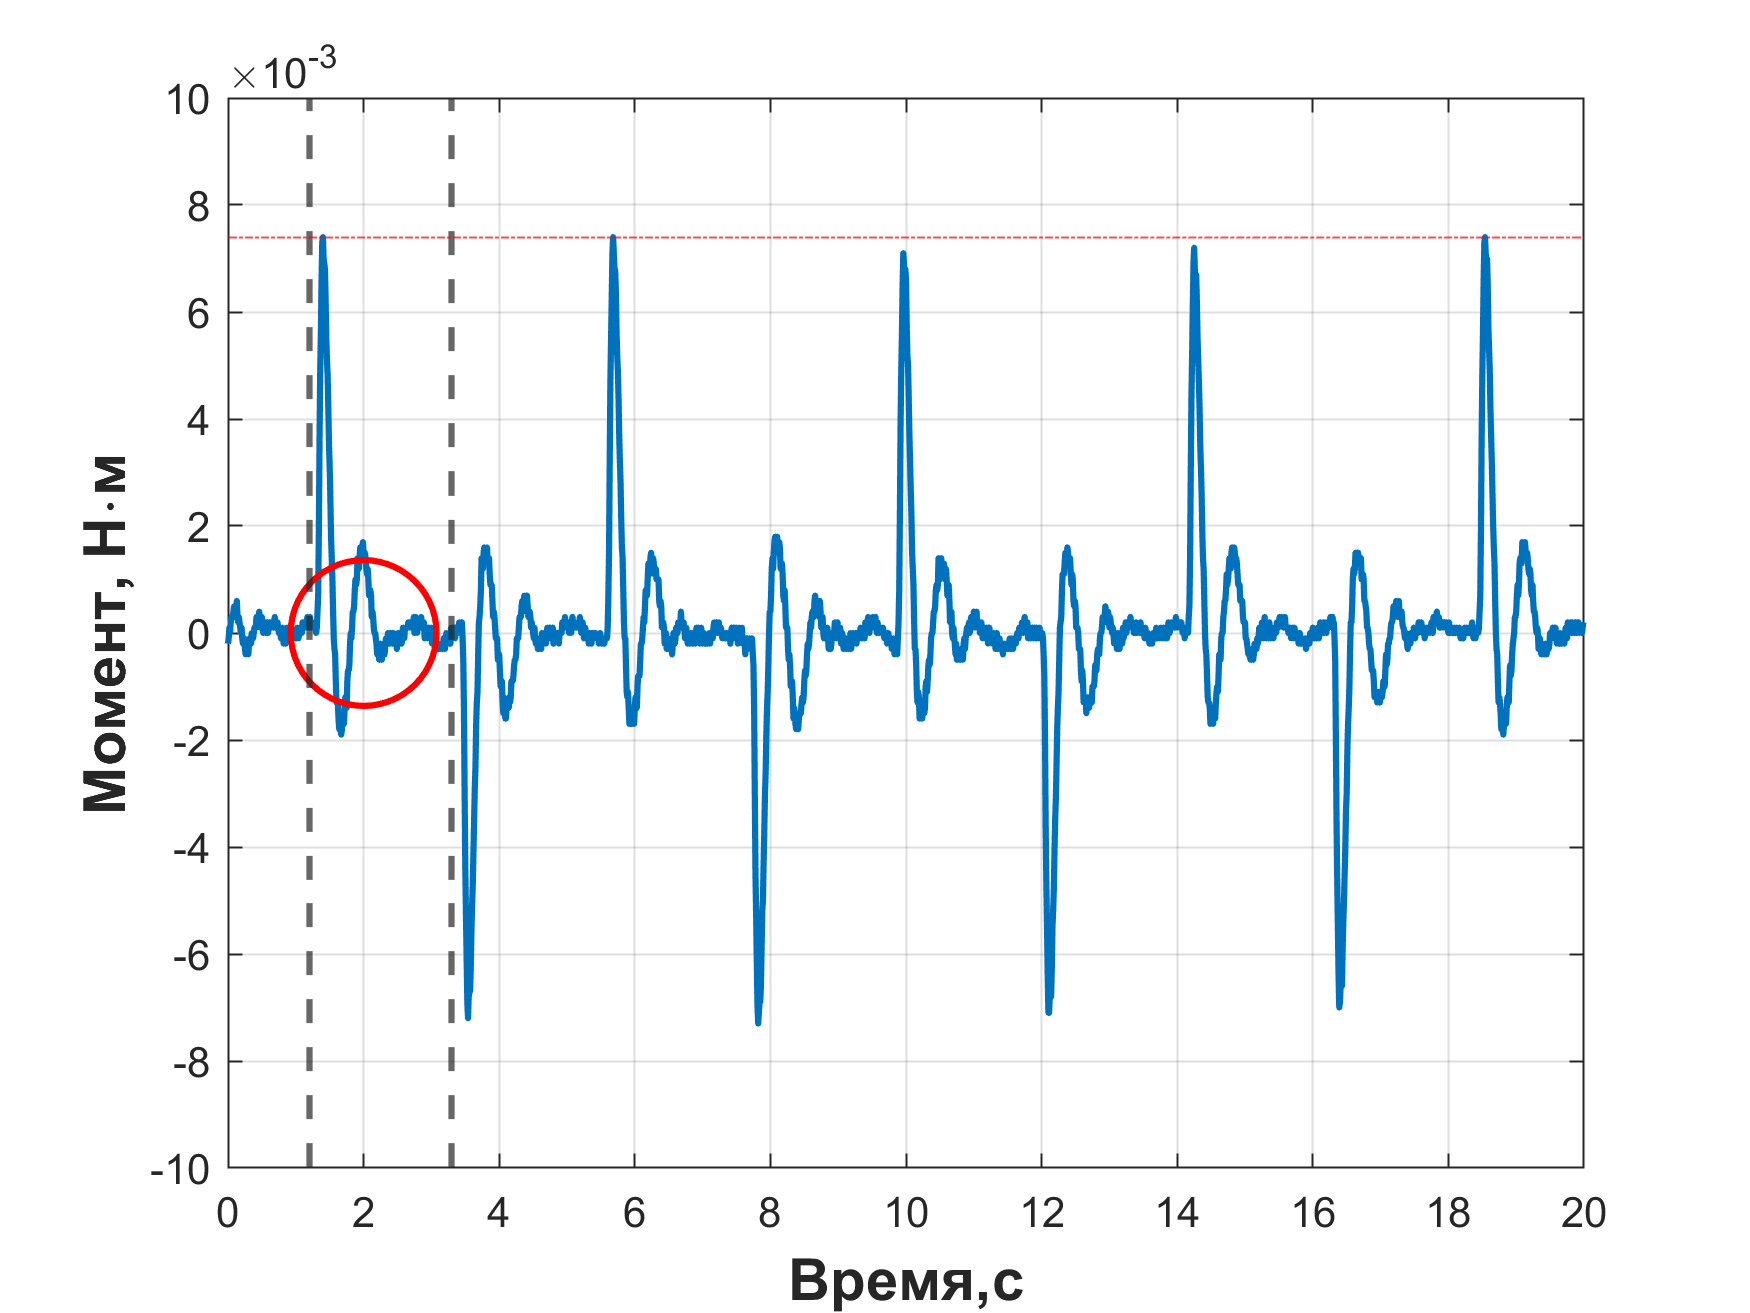
\includegraphics[width=1\linewidth]{matlab/img/scanner_no_sinchron} \\ а)
	\end{minipage}
	\hfill
	\begin{minipage}[b]{0.49\linewidth}\centering
		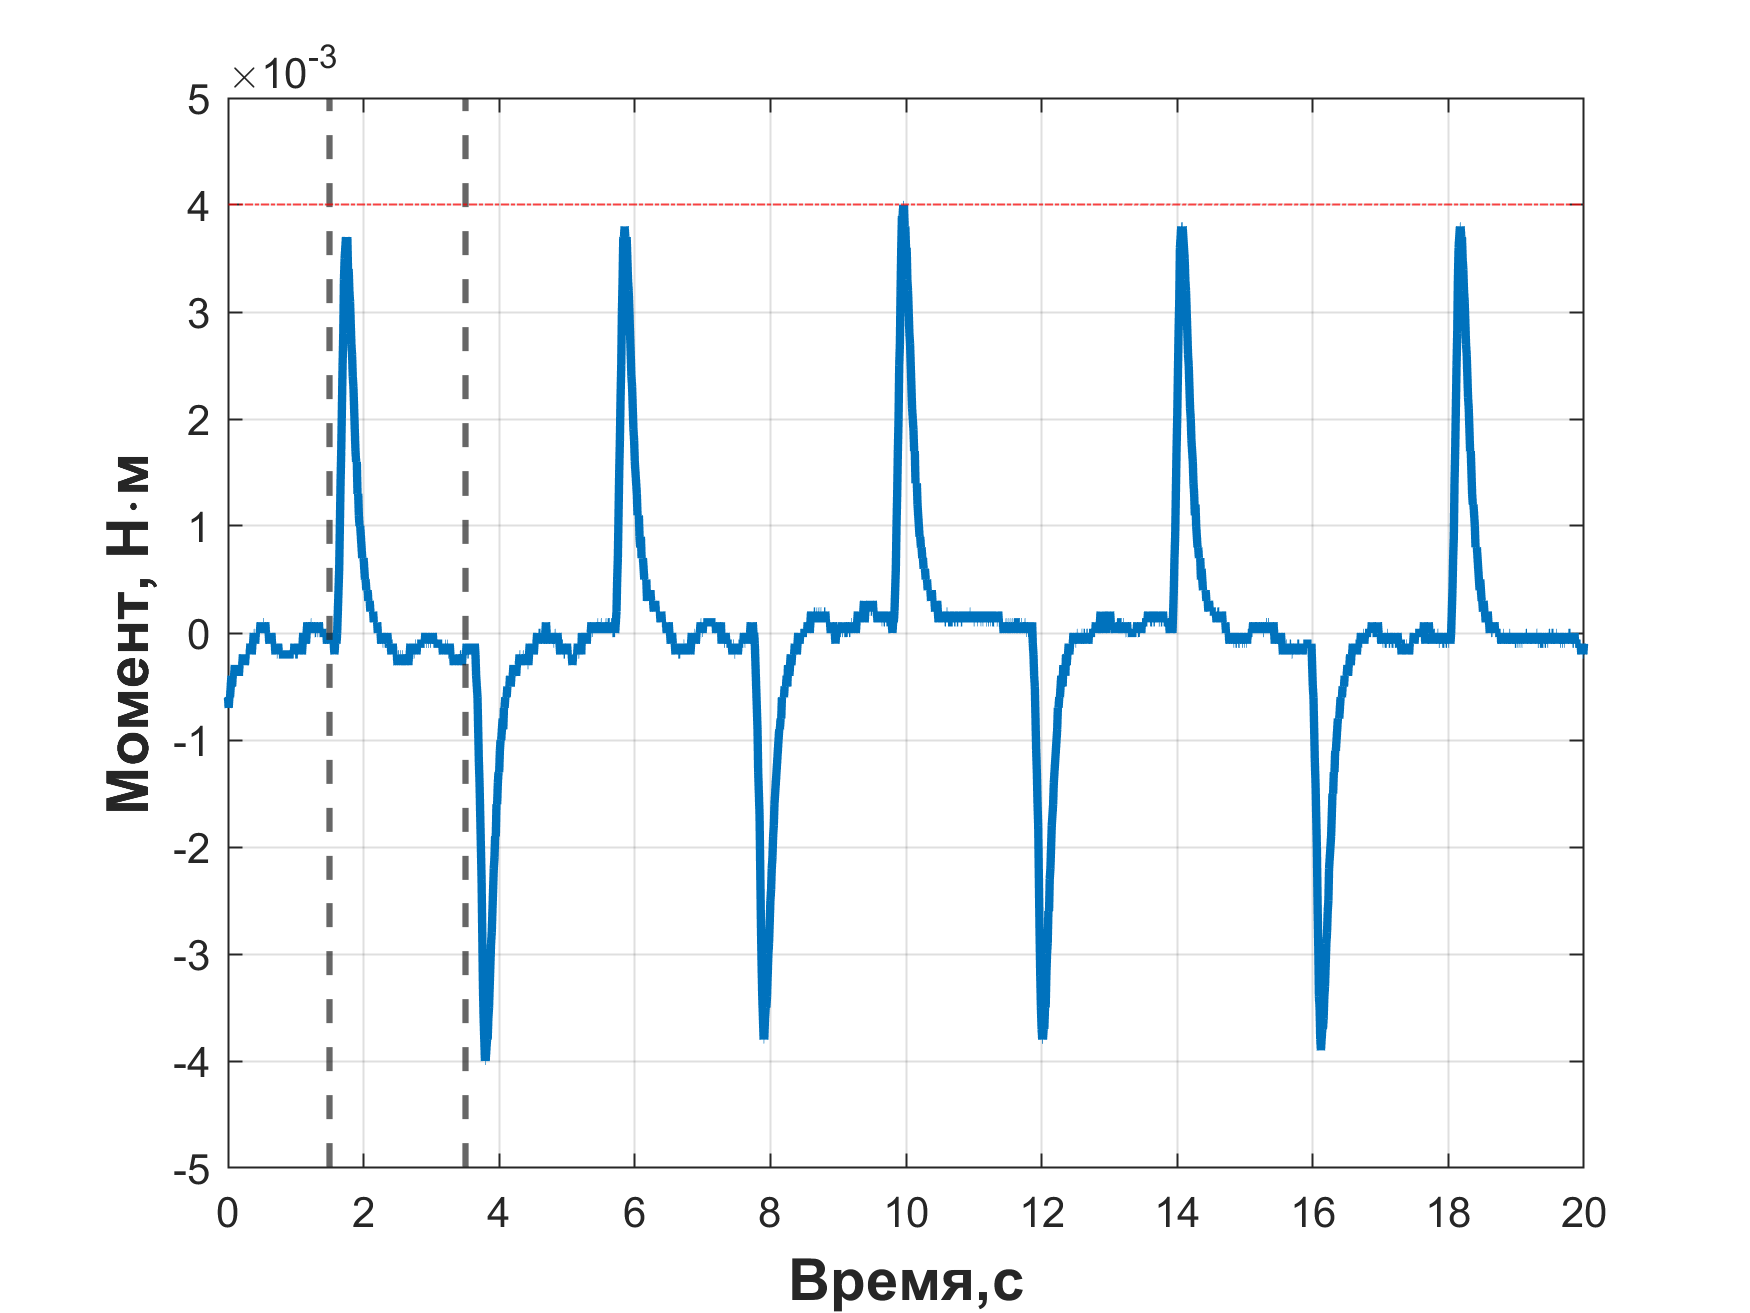
\includegraphics[width=1\linewidth]{matlab/img/scanner_correct} \\ б)
	\end{minipage}
	\caption{Реактивный момент оптической системы: а) до настройки; б) после настройки}
	\label{fig:scan-mom}
\end{figure}

Таким образом, стенд может применяться для настройки и отработки различных типов оптико-механических систем, обеспечивая снижение остаточного реактивного момента и повышение динамической точности.







\FloatBarrier
\pdfbookmark{Заключение}{conclusion}                                  % Закладка pdf
\section*{Заключение}
%% Согласно ГОСТ Р 7.0.11-2011:
%% 5.3.3 В заключении диссертации излагают итоги выполненного исследования, рекомендации, перспективы дальнейшей разработки темы.
%% 9.2.3 В заключении автореферата диссертации излагают итоги данного исследования, рекомендации и перспективы дальнейшей разработки темы.


В результате выполненных исследований достигнута цель работы — разработана и экспериментально подтверждена методика прямого измерения реактивных моментов, возникающих при работе оптико-механических систем космических аппаратов.

Анализ существующих подходов показал, что традиционные методы регистрации крутящего момента на валу двигателя не позволяют оценить суммарное воздействие на конструкцию и не учитывают динамических факторов, определяющих качество формируемого изображения.

Разработана математическая модель формирования реактивных моментов, учитывающая смещение центра масс, особенности конструкции карданового подвеса и компенсацию маховиками. Показано, что величина остаточного момента определяется как конструктивными параметрами, так и законом управления приводом. Обосновано применение синусоидального профиля разгона, обеспечивающего минимизацию энергии рывка и снижение уровня возбуждаемых колебаний.

Разработана и метрологически аттестована методика измерения реактивных моментов по угловым колебаниям подвесной системы, реализованная на созданном испытательном стенде. Аттестация подтвердила диапазон измеренийот $10^{-3}$ до $1\,\text{Н}\cdot\text{м}$ при относительной погрешности не более 2~\%.

Результаты стендовых испытаний показали хорошее совпадение с расчётными данными. Применение балансировочных колец и синусоидального профиля управления приводом позволило снизить уровень остаточных моментов и сгладить переходные процессы. Достоверность результатов подтверждена анализом данных бортовых гироскопов на лётных испытаниях.

Разработанная методика и созданный стенд могут использоваться для настройки и испытаний различных типов оптико-механических систем, включая устройства с дискретными и периодическими движениями. Это обеспечивает повышение динамической точности, снижение остаточного реактивного момента и улучшение качества изображений, формируемых космическими оптическими аппаратами.

\pdfbookmark{Литература}{bibliography}                                % Закладка pdf

\section*{Публикации в изданиях, рекомендованных ВАК России}
\begin{enumerate}
\item Стенд измерения остаточного реактивного момента оптико-механической системы / И.~М.~Белан, Ю.~П.~Ларионов, Д.~Ю.~Ларионов // Оптический журнал. "--- 2023. "--- Т.~90, №~7. "--- С.~60--67.

\item Ларионов Д.~Ю., Белан И.~М.  
Известия СПбГЭТУ «ЛЭТИ» // Известия. – 2024. – Т.~17. – №~7. – С.~16--22.




\end{enumerate}

\ifdefmacro{\microtypesetup}{\microtypesetup{protrusion=false}}{} % не рекомендуется применять пакет микротипографики к автоматически генерируемому списку литературы
\urlstyle{rm}                               % ссылки URL обычным шрифтом
\ifnumequal{\value{bibliosel}}{0}{% Встроенная реализация с загрузкой файла через движок bibtex8
    \renewcommand{\bibname}{\large \bibtitleauthor}
    \nocite{*}
    \insertbiblioauthor           % Подключаем Bib-базы
    %\insertbiblioexternal   % !!! bibtex не умеет работать с несколькими библиографиями !!!
}{% Реализация пакетом biblatex через движок biber
    % Цитирования.
    %  * Порядок перечисления определяет порядок в библиографии (только внутри подраздела, если `\insertbiblioauthorgrouped`).
    %  * Если не соблюдать порядок "как для \printbibliography", нумерация в `\insertbiblioauthor` будет кривой.
    %  * Если цитировать каждый источник отдельной командой --- найти некоторые ошибки будет проще.
    %


    \ifnumgreater{\value{usefootcite}}{0}{
        \begin{refcontext}[labelprefix={}]
            \ifnum \value{bibgrouped}>0
                \insertbiblioauthorgrouped    % Вывод всех работ автора, сгруппированных по источникам
            \else
                \insertbiblioauthor      % Вывод всех работ автора
            \fi
        \end{refcontext}
    }{
        \ifnum \totvalue{citeexternal}>0
            \begin{refcontext}[labelprefix=A]
                \ifnum \value{bibgrouped}>0
                    \insertbiblioauthorgrouped    % Вывод всех работ автора, сгруппированных по источникам
                \else
                    \insertbiblioauthor      % Вывод всех работ автора
                \fi
            \end{refcontext}
        \else
            \ifnum \value{bibgrouped}>0
                \insertbiblioauthorgrouped    % Вывод всех работ автора, сгруппированных по источникам
            \else
                \insertbiblioauthor      % Вывод всех работ автора
            \fi
        \fi
        %  \insertbiblioauthorimportant  % Вывод наиболее значимых работ автора (определяется в файле characteristic во второй section)
        \begin{refcontext}[labelprefix={}]
            \insertbiblioexternal            % Вывод списка литературы, на которую ссылались в тексте автореферата
        \end{refcontext}
        % Невидимый библиографический список для подсчёта количества внешних публикаций
        % Используется, чтобы убрать приставку "А" у работ автора, если в автореферате нет
        % цитирований внешних источников.
        \printbibliography[heading=nobibheading, section=0, env=countexternal, keyword=biblioexternal, resetnumbers=true]%
    }
}
\ifdefmacro{\microtypesetup}{\microtypesetup{protrusion=true}}{}
\urlstyle{tt}                               % возвращаем установки шрифта ссылок URL
